\section{Modellierung}
\label{sec3:model}
Dieses Kapitel widmet sich der konzeptuellen Modellierung und es werden, entsprechend der Methodik nach Nunamaker, alle Forschungsziele der Theoriebildungsphase behandelt.
Die Struktur dieses Kapitels folgt der logischen Abfolge der Forschungsziele.
Am Anfang wird in \cref{sec3:model:subsec:concept-modeling-methodology} die Konzeptions- und Modellierungsmethodik vorgestellt und beschrieben.
In \cref{sec3:model:subsec:fz-explainability} wird das Forschungsziel \enquote{FZ 1.2/TB Erklärbarkeit von MMIR mittels generativer KI} behandelt und es werden Möglichkeiten der Erklärbarkeit durch generative KI angesprochen, sowie Anwendungsfälle von Benutzern als Basis für weitere Modellierungsvorgehen identifiziert.
In \cref{sec3:model:subsec:fz-integration} wird das Forschungsziel \enquote{FZ 2.2/TB Integration generativer KI in das GMAF} behandelt und es werden die technischen Aspekte der Integration von Systemen generativer KI besprochen.
Dies umfasst die Überführung von Gaph Codes in eine passende Form der Eingabe für Systeme generativer KI und verwandte Aspekte, sowie die Integration der verfügbaren Endpunkte der von den ausgewählten Systemen angebotenen Schnittstelle.
Am Ende jedes Forschungsziels werden die Erkenntnisse aus diesen Bereichen diskutiert und das weitere Vorgehen festgehalten.
Abschließend wird in \cref{sec3:model:subsec:summary} eine Zusammenfassung der in diesem Kapitel erarbeiteten Ergebnisse gegeben.

{
    \def\arraystretch{1.1}%
    \begin{xltabular}{\linewidth}{
            @{}
            >{
                \hsize=0.25\linewidth
                \raggedright\arraybackslash
            }X
            >{
                \hsize=0.55\linewidth
                \raggedright\arraybackslash
            }X
            >{
                \hsize=0.2\linewidth
                \centering\arraybackslash
            }X
            @{}
    }

    % First Header

    \caption{Struktur dieses Kapitels.}
    \label{sec3:model:table:structure} \\

    \toprule

    \textbf{FZ} & \textbf{Kurze Beschreibung} & \textbf{Abschnitt} \\

    \midrule

    \endfirsthead

    % Normal Head

    \toprule

    \textbf{FZ} & \textbf{Kurze Beschreibung} & \textbf{Abschnitt} \\

    \midrule

    \endhead

    % Lower Rows

    Konzeptions- und Modellierungsmethodik & Konzeptuelle Gestaltung der Modellierung & \cref{sec3:model:subsec:concept-modeling-methodology} \\
    FZ 1.2/TB & Modellierung: Erklärbarkeit \& gen. KI & \cref{sec3:model:subsec:fz-explainability} \\
    FZ 2.2/TB & Modellierung: Integration generativer KI & \cref{sec3:model:subsec:fz-integration} \\
    Zusammenfassung & Ergebnisse / Erkenntnisse & \cref{sec3:model:subsec:summary} \\

    \bottomrule

    \end{xltabular}
}


\subsection{Konzeptions- und Modellierungsmethodik}
\label{sec3:model:subsec:concept-modeling-methodology}
Die konzeptuelle Gestaltung und Modellierung in diesem Kapitel folgt dem Paradigma \enquote{User Centered System Design} \cite{norman-draper-user-centered-system-design} von Norman \& Draper.
Ziel dieses Paradigmas ist eine Modellierung aus der Perspektive eines Benutzers oder eines Anwendungsfalls.
Die konzeptuelle Gestaltung folgt dem Vorgehen des Rational Unified Process (RUP) \cite{rup-quality} und wird mittels der Unified Modeling Language beschrieben \cite{rup-inff}.

\subsubsection{Rational Unified Process}
\label{sec3:model:subsubsec:rup}
Der Rational Unified Process (RUP) ist ein für die Nutzung der Modellierungssprache Unified Modeling Language (UML) beschriebenes Vorgehensmodell bzw. Phasenmodell für die Anwendungsentwicklung \cite{rup-inff}.
Das Vorgehensmodell des RUP wird dabei in UML beschrieben \cite{rup-inff}.
Der Arbeitsablauf im RUP-Vorgehensmodell leitet sich aus dem evolutionären bzw. inkrementellen Vorgehen ab und lässt sich in vier zeitlich geordnete Phasen und Iterationen jener aufteilen:
\textit{Planung, Ausarbeitung, Errichtung, Übergang} \cite{rup-inff}.
Die Struktur der Phasen und der Iterationen im RUP-Vorgehensmodell werden durch sechs Kernarbeitsprozesse abgedeckt \cite{rup-inff}:
\begin{itemize}
    \item Geschäfts- und Modellierungskonzept
    \item Anforderungen
    \item Analyse \& Design
    \item Implementierung
    \item Test
    \item Inbetriebnahme
\end{itemize}

\begin{figure}[htb]
    \centering
    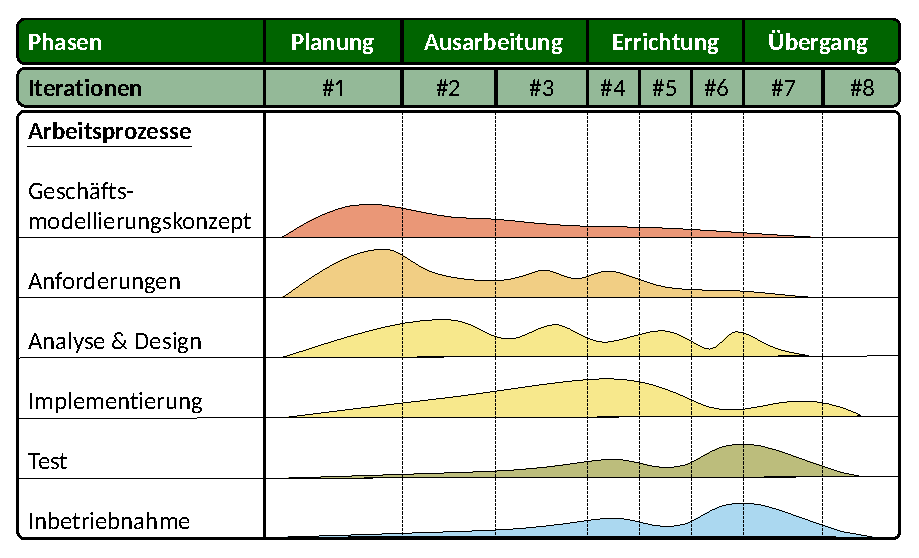
\includegraphics{chapter/chapter_3/rup.eps}
    \caption{Modellierung zum Vorgehen des Rational Unified Process.}
    \label{sec3:model:subsec:conc-model-metho:fig:rup}
\end{figure}

Die Kern-Arbeitsprozesse \enquote{Geschäfts-Modellierungskonzept}, \enquote{Anforderungen} und \enquote{Analyse \& Gestaltung} sind Teil dieses Kapitels und setzen die Methodik für die Bearbeitung der Forschungsziele der Theoriebildungsphase nach Nunamaker um.
Der Arbeitsprozess \enquote{Implementierung} des RUP-Vorgehensmodells entspricht den Forschungszielen der Implementierungsphase nach Nunamaker und wird in \cref{sec4:impl} behandelt.
Der Arbeitsprozess \enquote{Test} des RUP-Vorgehensmodells entspricht den Forschungszielen der Experimentphase nach Nunamaker und wird in \cref{sec5:eval} behandelt. Der Arbeitsprozess \enquote{Inbetriebnahme} wird in dieser Arbeit nicht behandelt. Somit wird jeder konzeptionelle Entwurf und jede Modellierung aus der Perspektive eines Benutzers oder eines Anwendungsfalls und auf Grundlage der Arbeitsprozesse des RUP-Vorgehensmodells entwickelt und im weiteren Verlauf dieser Arbeit unter Verwendung der UML formalisiert. Dabei
ist es Ziel der Modellierung wiederverwendbare Softwarekomponenten zu erstellen, die erweiterbar, konfigurierbar sowie wartbar sind. Die Auswahl der Konzeptions- und Modellierungsmethodiken erfordert eine spezielle Anordnung der Forschungsziele. Diese Anordnung sieht wie folgt aus:
\begin{itemize}
    \item FZ 1.2/TB Erklärbarkeit von MMIR mittels generativer KI
    \item FZ 2.2/TB Integration generativer KI in das GMAF
\end{itemize}
Die Notwendigkeit dieser Anordnung ergibt sich nach der Methodik von Norman \& Draper, in welcher die Modellierung aus der Perspektive eines Benutzers oder eines Anwendungsfalls beginnt. Des Weiteren bauen die ersten Kern-Arbeitsprozesse \enquote{Geschäfts-Modellierungskonzept} und \enquote{Anforderungen} des RUP-Vorgehensmodells auf Anwendungsfällen auf. Somit ist logischer Startpunkt die Erklärbarkeit von MMIR mittels generativer KI.

\FloatBarrier

\subsubsection{Unified Modeling Language}
\label{sec3:model:subsubsec:uml}
Die Unified Modeling Language (UML) \cite{omg-uml} ist eine standardisierte, visuelle Modellierungssprache, die ihre Verwendung in der Softwareentwicklung findet \cite{visual-paradigm-uml}.
UML kann allerdings auch in anderen technischen Bereichen, oder der Geschäftsmodellierung verwendet werden \cite{Kreische2004}.
Die UML hat zum Ziel, komplexe Systeme und deren Prozesse grafisch darzustellen, zu analysieren, zu spezifizieren und zu dokumentieren \cite{visual-paradigm-uml}.
Die UML wurde dazu entwickelt, um die Kommunikation zwischen Softwareentwicklern, Analysten, Designern und anderen involvierten Parteien bzw. Interessensgruppen zu erleichtern \cite{visual-paradigm-uml}.
Um diese Kommunikation zu ermöglichen, bietet die UML eine Vielzahl von Diagrammtypen zur einheitlichen, verständlichen und flexiblen Darstellung von Systemstrukturen- und verhalten.
Folgende Aufzählung umfasst die bekanntesten und am häufigsten verwendeten Diagrammtypen, sowie ihre jeweiligen Aufgaben.
\begin{itemize}
    \item Klassendiagramm: Stellt die simple, statische Struktur eines Systems durch seine Klassen, Attribute, Methoden und deren Beziehungen untereinander dar.
    \item Anwendungsfalldiagramm: Stellt die Interaktion zwischen Akteuren, die Benutzer oder widerum andere Systeme sein können, und dem System dar.
    Zweck ist die Darstellung der für die Akteure verfügbaren Funktionalitäten des Systems.
    \item Sequenzdiagramm: Stellt die Interaktion zwischen Objekten eines Systems in einem zeitlichen Verlauf dar.
    Interaktion geschieht durch das Senden von Nachrichten zwischen den Objekten.
    \item Aktivitätsdiagramm: Stellt den Ablauf von Aktivitäten und Prozessen dar, um den Kontrollfluss innerhalb eines Systems zu visualisieren.
    \item Zustandsdiagramm: Stellt den Lebenszyklus eines Objekts dar und zeigt auf, wie es auf Ereignisse und Zuständsänderungen reagiert.
\end{itemize}
Die wichtigste Eigenschaft der UML ist seine Unabhängigkeit zu spezifischen Technologien, wie z.B. Programmiersprachen \cite{ibm-uml}.
Diese Eigenschaft ermächtigt die UML zur Modellierung verschiedenster Systeme in vielen unterschiedlichen Bereichen.
Bekannte Beispiele sind Softwareanwendungen, Datenbanken und Geschäftsprozesse.
Mittels eines wohl definierten, sowie gepflegten Standards, der durch die OMG \cite{omg} erfolgt und eine einheitliche Sprache für Kommunikation schafft, ermöglicht die UML eine nahtlose Zusammenarbeit zwischen verschiedensten involvierten Gruppen.
Angesichts dieser Eigenschaft ist die Unified Modeling Language ein wertvolles Werkzeug für die Softwaremodellierung- und entwicklung komplexer Systeme.

\clearpage

\subsection[FZ 1.2/TB Erklärbarkeit von MMIR mittels generativer KI]{\texorpdfstring{FZ 1.2/TB Erklärbarkeit von MMIR mittels \\ generativer KI}{FZ 1.2/TB Erklärbarkeit von MMIR mittels generativer KI}}
\label{sec3:model:subsec:fz-explainability}
Dieser Abschnitt befasst sich mit der Modellierung der \enquote{Erklärbarkeit von MMIR mittels generativer KI}.
Dabei werden die in \hyperref[sec2:sota:subsec:fz-explainability]{FZ 1.1/O} identifizierten, offenen Herausforderungen \hyperref[sec2:sota:oi:1.1]{\textbf{OH 1.1}} und \hyperref[sec2:sota:oi:1.2]{\textbf{OH 1.2}} adressiert.
Ziel dieses Abschnitts ist es Konzepte für den Einsatz von Systeme generativer KI für Erklärbarkeit hervorzubringen und Anwendungsfälle zur Interaktion mit selbigen zu identifizieren.
Hierzu wird in \cref{sec3:model:subsubsec:explainability-through-genai} die offene Herausforderung \hyperref[sec2:sota:oi:1.1]{\textbf{OH 1.1}} und in \cref{sec3:model:subsubsec:use-cases} die offene Herausforderung \hyperref[sec2:sota:oi:1.2]{\textbf{OH 1.2}} adressiert.

\subsubsection{Erklärbarkeit durch generative KI}
\label{sec3:model:subsubsec:explainability-through-genai}
In diesem Abschnitt wird die erste offene Herausforderung \hyperref[sec2:sota:oi:1.1]{\textbf{OH 1.1}} adressiert und es werden mögliche Techniken zum Erzeugen von Erklärungen durch generative KI angesprochen.
In \cref{sec2:sota:par:basic-concepts} wurde das Konzept des Prompt Engineering erklärt und eine Reihe an Techniken, sowie dazugehörige Beispiele präsentiert.
Um mit Hilfe von Systemen generativer KI Erklärungen generieren zu können, müssen die Eingaben in ein System möglichst präzise formuliert sein.
Ziel muss es daher sein, mit gezielten und präzise formulierten Eingabeaufforderungen das System so zu instruieren, dass es möglichst genaue Erklärungen generieren kann.
In \cite{zero-shot-reasoners} wurde bereits gezeigt, dass das recht simple Textanhängsel \enquote{Lets think step by step.} einen großen Einfluss auf die Schlussfolgerungen und somit auch die Ausgabe einer generativen KI haben kann.
Es ist daher nicht abwegig anzunehmen, dass eine simple Instruktion, wie z.B. \enquote{Create a coherent textual explanation.} oder \enquote{Create a visual explanation.} einen positiven Einfluss auf erzeugte Texte bzw. Erklärungen haben könnte.
Eine weitere interessante Idee Erklärungen generieren zu lassen, wäre die Methode des Geschichtenerzählens.
Eine beispielhafte Instruktion könnte sein: \enquote{Make up a story.}.
Weitere \enquote{elementare Bausteine} einer Instruktion können dann beispielhafte Erklärungen umfassen, um dem System zu zeigen, welche Art von Erklärung letztlich gewünscht wird, oder die Vorgabe eines unvollständigen Satzes, welcher dann vom System komplementiert wird.

\subsubsection{Anwendungsfälle}
\label{sec3:model:subsubsec:use-cases}
Ein sinnvoller Einsatz von Systemen generativer KI im GMAF zur Erklärung von Graph Codes setzt eine Benutzerschnittstelle mit geeigneten Interaktionsmöglichkeiten voraus.
In diesem Abschnitt wird die zweite offene Herausforderung \hyperref[sec2:sota:oi:1.2]{\textbf{OH 1.2}} adressiert und es werden eine Reihe an Anwendungsfällen aus der Perspektive von Benutzern bzw. Anwendern des GMAF identifiziert und beschrieben.
\cref{sec3:model:subsubsec:use-cases:fig:overview-use-cases} zeigt ein UML-Diagramm zur Übersicht der identifizierten Anwendungsfälle.
\begin{figure}[htb]
    \centering
    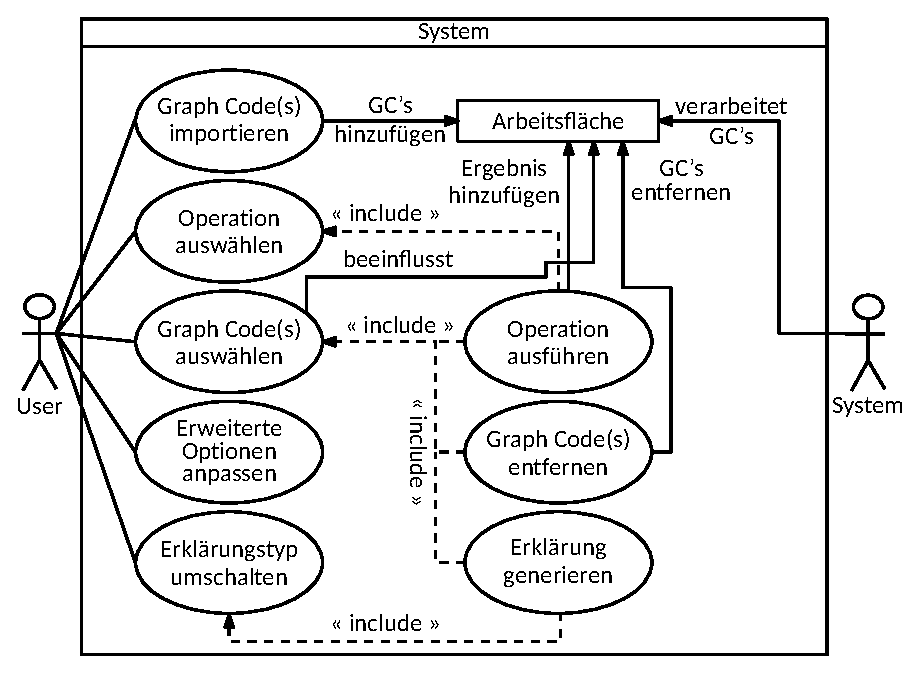
\includegraphics[width=\textwidth]{chapter/chapter_3/uml-explainer-system.eps}
    \caption{Übersicht über alle Anwendungsfälle.}
    \label{sec3:model:subsubsec:use-cases:fig:overview-use-cases}
\end{figure}
\noindent
Diese identifizierten Anwendungsfälle stellen die Basis für weitere Modellierungsvorgehen dar und werden im Laufe dieses Abschnitts weiter ausgeführt.
Weitere Ausführungen umfassen textuelle Beschreibungen, erste Wireframes, die das allgemeine Skelett der Anwendung darstellen sollen, Mechanismen, die die an Anwendungsfällen beteiligten Komponenten identifizieren, sowie Sequenzdiagramme, um die Interaktion zwischen den Objekten bzw. Komponenten eines Systems darzustellen.
Anhand dieser Modellierungsvorgehen werden die Wireframes weiter ausgeführt bzw. ausgebaut.

\paragraph{Textuelle Beschreibungen}
\label{sec3:model:par:textual-desc-use-cases}
In diesem Abschnitt werden die in \cref{sec3:model:subsubsec:use-cases:fig:overview-use-cases} dargestellten Anwendungsfälle detailliert beschrieben.
Diese detaillierte Beschreibung umfasst jeweils eine Beschreibung der Aufgabe des Anwendungsfalles, die Akteure, die an diesem Anwendungsfall beteiligt sind, die Vorbedingungen, die vor dem Anwendungsfall gelten, einen Ablauf an Schritten zum Durchführen des Anwendungsfalls und schlussendlich die Nachbedinungen, die jeweils nach dem Anwendungsfall gelten.

\begin{usecase}{UC-1.1 Graph Code(s) importieren}
\label{sec3:model:uc-1.1}
    \desc{
        Benutzer klicken in der Arbeitsfläche einen Knopf \enquote{Select Graph Code(s)}.
        Daraufhin öffnet sich ein Filechooser, in welchem Benutzer eine Auswahl von einem oder mehrerer Graph Code Datei(en) treffen können.
        Die ausgewählten Graph Code Datei(en) werden einer Liste in der Arbeitsfläche hinzugefügt und angezeigt.
    }
    \tcbline
    \actors{Benutzer, System}
    \tcbline
    \pre{Keine.}
    \tcbline
    \mainflow{
        \item System zeigt eine Liste in der Arbeitsfläche an.
        \item Benutzer klickt Knopf \enquote{Select Graph Code(s).}
        \item System zeigt Filechooser an.
        \item Benutzer wählt ein oder mehrere Graph Code Datei(en) aus.
        \item System fügt Graph Code Datei(en) der Liste in der Arbeitsfläche zu.
    }
    \tcbline
    \post{Graph Code Datei(en) sind der Liste in der Arbeitsfläche hinzugefügt worden.}
\end{usecase}

\begin{usecase}{UC-1.2 Graph Code(s) entfernen}
\label{sec3:model:uc-1.2}
    \desc{
        Benutzer wählen aus der Liste in der Arbeitsfläche ein oder mehrere Graph Code Datei(en) aus und können über einen Knopf \enquote{Remove selected Graph Code(s)} diese Graph Codes aus der Liste und somit der Arbeitsfläche entfernen.
    }
    \tcbline
    \actors{Benutzer, System}
    \tcbline
    \pre{
        \begin{itemize}
            \item Liste enthält ein oder mehrere Graph Code(s).
            \item Benutzer haben ein oder mehrere Graph Code(s) ausgewählt.
        \end{itemize}
    }
    \tcbline
    \mainflow{
        \item System zeigt eine Liste an Graph Codes in der Arbeitsfläche an.
        \item Benutzer wählt ein oder mehrere Graph Code(s) aus.
        \item Benutzer klickt auf Knopf \enquote{Remove selected Graph Code(s).}
        \item System entfernt ausgewählte Graph Codes aus der Liste in der Arbeitsfläche.
    }
    \tcbline
    \post{Ausgewählte Graph Code Datei(en) sind aus der Liste in der Arbeitsfläche entfernt worden.}
\end{usecase}

\begin{usecase}{UC-1.3 Graph Code(s) auswählen}
\label{sec3:model:uc-1.3}
    \desc{
        Benutzer wählen aus der Liste in der Arbeitsfläche ein oder mehrere Graph Code Datei(en) aus.
        Die Auswahl von Graph Code Dateien dient als Grundlage für Anwendungsfälle, wie \hyperref[sec3:model:uc-1.2]{UC-1.2}, \hyperref[sec3:model:uc-1.5]{UC-1.5} oder \hyperref[sec3:model:uc-1.8]{UC-1.8}.
    }
    \tcbline
    \actors{Benutzer, System}
    \tcbline
    \pre{
        Liste enthält ein oder mehrere Graph Code(s) zum Auswählen.
    }
    \tcbline
    \mainflow{
        \item System zeigt eine Liste an Graph Code(s) in der Arbeitsfläche an.
        \item Benutzer wählen ein oder mehrere Graph Code(s) an.
    }
    \tcbline
    \post{Keine.}
\end{usecase}

\begin{usecase}{UC-1.4 Operation auswählen}
\label{sec3:model:uc-1.4}
    \desc{
        Benutzer wählen aus einem Feld eine auszuführende Operation aus.
        Verfügbare Optionen sind: Vereinigung, Subtraktion, Gemeinsamkeiten, Unterschiede.
        Das Auswählen einer Operation ist die Vorbedingung für den Anwendungsfall \hyperref[sec3:model:uc-1.5]{UC-1.5}, dem Ausführen einer Operation.
    }
    \tcbline
    \actors{Benutzer, System}
    \tcbline
    \pre{Keine.}
    \tcbline
    \mainflow{
        \item System bietet in einem Feld eine Reihe an auszuwählenden Operationen.
        \item Benutzer wählt eine Operation aus.
    }
    \tcbline
    \post{Keine.}
\end{usecase}

\begin{usecase}{UC-1.5 Operation ausführen}
\label{sec3:model:uc-1.5}
    \desc{
        Benutzer klicken auf den Knopf \enquote{Execute}, um die vorher ausgewählte Operation auf den in der Arbeitsfläche ausgewählten Graph Code Datei(en) auszuführen.
        Die vorher ausgewählte Operation wird daraufhin auf den ausgewählten Graph Code Datei(en) ausgeführt.
    }
    \tcbline
    \actors{Benutzer, System}
    \tcbline
    \pre{
        \begin{itemize}
            \item Operation in der Arbeitsfläche ausgewählt.
            \item In der Arbeitsfläche wurden Graph Code Datei(en) ausgewählt.
        \end{itemize}
    }
    \tcbline
    \mainflow{
        \item Benutzer klickt auf Knopf \enquote{Execute}.
        \item System führt vorher ausgewählte Operation auf den ausgewählten Graph Code Datei(en) aus.
    }
    \tcbline
    \post{Erfolgreich ausgeführte Operation auf ausgewählten Graph Code(s).}
\end{usecase}

\begin{usecase}{UC-1.6 Erklärungstyp umschalten}
\label{sec3:model:uc-1.6}
    \desc{
        Benutzer wählen in der Arbeitsfläche über Knöpfe \enquote{Image} oder \enquote{Text} den Typ der Erklärung aus.
        Anhand der ausgewählten Erklärung wird die Benutzerschnittstelle in der Arbeitsfläche für den jeweiligen Erklärungstyp umgeschaltet.
    }
    \tcbline
    \actors{Benutzer, System}
    \tcbline
    \pre{Keine.}
    \tcbline
    \mainflow{
        \item Benutzer wählen über die Knöpfe \enquote{Image} oder \enquote{Text} den Typ der Erklärung aus.
        \item System schaltet auf für Typ spezifische Benutzerschnittstelle um.
    }
    \tcbline
    \post{Benutzerschnittstelle für spezifischen Erklärungstyp umgeschaltet.}
\end{usecase}

\begin{usecase}{UC-1.7 Erweiterte Optionen anpassen}
\label{sec3:model:uc-1.7}
    \desc{
        Benutzer passen in einem dafür vorgesehenen Feld erweiterte Optionen für den Endpunkt, der für die zu generierende Erklärung zuständig ist, an.
        Die anpassbaren Optionen sind abhängig vom jeweiligen Endpunkt bzw. Erklärungstypen.
    }
    \tcbline
    \actors{Benutzer, System}
    \tcbline
    \pre{Keine.}
    \tcbline
    \mainflow{
        \item System bietet, abhängig vom Endpunkt bzw. Erklärungstypen, eine Reihe an anpassbaren Optionen an.
        \item Benutzer passen Optionen nach eigenen Bedürfnissen an.
    }
    \tcbline
    \post{Keine.}
\end{usecase}

\begin{usecase}{UC-1.8 Erklärung generieren}
\label{sec3:model:uc-1.8}
    \desc{
        Benutzer klicken auf einen Knopf \enquote{Generate ...}, um eine Erklärung für eine zuvor ausgewählte Graph Code Datei zu generieren.
        Die generierte Erklärung ist abhängig vom zuvor gewählten Endpunkt bzw. Erklärungstypen.
    }
    \tcbline
    \actors{Benutzer, System}
    \tcbline
    \pre{Graph Code Datei wurde ausgewählt.}
    \tcbline
    \mainflow{
        \item Benutzer klickt auf Knopf \enquote{Generate ...}
        \item System lässt durch Endpunkt Erklärung generieren.
        \item System zeigt Erklärung in einem dafür vorgesehenen Bereich der Benuzterschnittstelle an.
    }
    \tcbline
    \post{Keine.}
    \tcbline
    % Hier im Branchflow zwischen Image und Text differenzieren.
    \branchflow{
        \setcounter{enumi}{2}
        \item[\number\value{enumi}.a] Endpunkt für \enquote{Image} generiert eine visuelle Erklärung bzw. ein Bild.
        \item[\number\value{enumi}.b] Endpunkt für \enquote{Text} generiert eine textuelle Erklärung.
    }
\end{usecase}

\paragraph{Wireframe für die Interaktion mit Graph Codes}
\label{sec3:model:par:wireframe}
Auf Basis der Anwendungsfälle und den textuellen Beschreibungen dieser, wird in diesem Abschnitt ein Wireframe, sprich ein Konzept für eine Benutzerschnittstelle, vorgestellt.
\cref{sec3:model:par:wireframe:fig:stage-1} zeigt eine erste Ausführung eines Wireframes, welches die Grundbereiche und somit das Skelett der Benutzerschnittstelle darstellen soll.

\begin{figure}[htb]
    \centering
    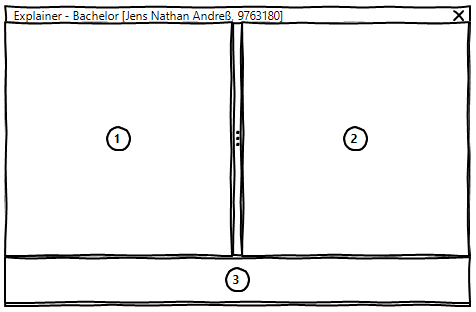
\includegraphics{chapter/chapter_3/wireframe-stage-1.png}
    \caption{Wireframe für die Grundbereiche der Benutzerschnittstelle.}
    \label{sec3:model:par:wireframe:fig:stage-1}
\end{figure}

In dieser Abbildung sind drei Grundbereiche zu erkennen, die im Folgenden genauer beschrieben werden:
\begin{enumerate}
    \item[\circitem{1}] ist der Bereich der Arbeitsfläche, in der die Bearbeitung von Graph Code Dateien stattfindet.
    Bearbeitungen von Graph Codes umfassen das Importieren, Auswählen und Entfernen von Graph Code Dateien, sowie das Auswählen und Ausführen von Operationen auf Graph Code Dateien.
    \item[\circitem{2}] ist der Bereich der Arbeitsfläche, in der Benutzer Erklärungen generieren können.
    Benutzer können hier zwischen unterschiedlichen Typen an Erklärungen hin und her schalten.
    \item[\circitem{3}] ist eine Konsole, in der alle wichtigen Informationen über Aktionen und Prozesse festgehalten werden.
\end{enumerate}
Anhand der Anwendungsfälle \hyperref[sec3:model:uc-1.1]{UC-1.1} bis \hyperref[sec3:model:uc-1.5]{UC-1.5} können in der linken Arbeitsfläche, die der Bearbeitung von Graph Codes dienen soll, wichtige Komponenten in der Benutzerschnittstelle identifiziert werden.
Analog können anhand der Anwendungsfälle \hyperref[sec3:model:uc-1.6]{UC-1.6} bis \hyperref[sec3:model:uc-1.8]{UC-1.8} in der rechten Arbeitsfläche, die sich der Erklärung von Graph Code Dateien widmet, weitere wichtige Komponenten in der Benutzerschnittstelle identifiziert werden.
\cref{sec3:model:par:wireframe:fig:stage-2+3} zeigt die linke und rechte Arbeitsfläche mit diesen neuen Komponenten in jeweils einem partiellen Wireframe.

\begin{figure}[htb]
    \centering
    \begin{minipage}[b]{.5\textwidth}
        \centering
        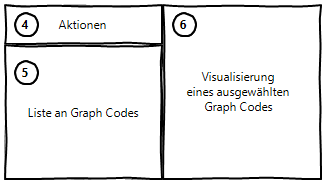
\includegraphics[width=\textwidth]{chapter/chapter_3/wireframe-stage-2.png}
    \end{minipage}%
    \begin{minipage}[t]{.5\textwidth}
        \centering
        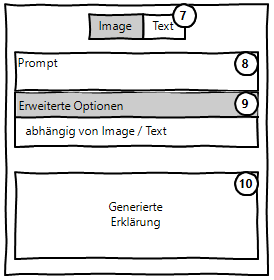
\includegraphics[width=0.9\textwidth]{chapter/chapter_3/wireframe-stage-3.png}
    \end{minipage}
    \caption{Wireframe für den linken Arbeitsbereich (links) und den rechten Arbeitsbereich (rechts) der Benutzerschnittstelle.}
    \label{sec3:model:par:wireframe:fig:stage-2+3}
\end{figure}

Diese neuen Komponenten werden im Folgenden genauer beschrieben:
\begin{enumerate}
    \item[\circitem{4}] ist der Aktionsbereich, in welchem Interaktionsmöglichkeiten, wie das Importieren und Entfernen von Graph Codes in die Arbeitsfläche eingebunden werden.
    Des Weiteren werden in diesem Aktionsbereich auch Interaktionsmöglichkeiten für die Auswahl und das Ausführen von Operationen auf den zuvor in der Arbeitsfläche ausgewählten Graph Code Dateien eingebunden.
    \item[\circitem{5}] ist der Bereich in der Benutzerschnittstelle, in der die Graph Code Dateien in einer Liste dargestellt werden.
    Diese Liste ist die Voraussetzung für Anwendungsfälle \hyperref[sec3:model:uc-1.2]{UC-1.2}, \hyperref[sec3:model:uc-1.3]{UC-1.3}, \hyperref[sec3:model:uc-1.5]{UC-1.5} und \hyperref[sec3:model:uc-1.8]{UC-1.8}.
    \item[\circitem{6}] ist der Bereich der Benutzerschnittstelle, in der ausgewählte Graph Code Datei(en) in einer geeigneten Form visualisiert werden.
    Da Graph Codes quadratische Matrizen sind, eignet sich für die visuelle Form der Darstellung eine Tabelle.
    \item[\circitem{7}] sind die Knöpfe, mit welchen Benutzer zwischen den Benutzerschnittstellen für die jeweiligen Erklärungstypen umschalten können.
    \item[\circitem{8}] ist die Prompt, die später über den entsprechenden Endpunkt in das System generativer KI übermittelt werden soll.
    \item[\circitem{9}] zeigt erweiterte anpassbare Optionen für den jeweiligen Endpunkt.
    \item[\circitem{10}] ist der Bereich, in welchem das Endergebnis der Anfrage an das System generativer KI dargestellt wird.
\end{enumerate}
Zusammengeführt ergeben diese partiellen Wireframes ein ganzes Wireframe, welches in \cref{sec3:model:par:wireframe:fig:complete-stage} abgebildet ist und die komplette Benutzerschnittstelle darstellt.

\begin{figure}[htb]
    \centering
    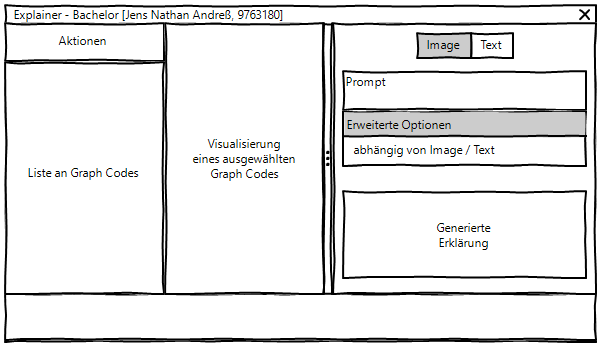
\includegraphics[width=\textwidth]{chapter/chapter_3/wireframe-complete-stage.png}
    \caption{Komplettes Wireframe für die Benutzerschnittstelle.}
    \label{sec3:model:par:wireframe:fig:complete-stage}
\end{figure}
Die in diesem Abschnitt dargestellten Wireframes bilden die Struktur der Benutzerschnittstelle und werden im weiteren Verlauf dieser Arbeit in \hyperref[sec4:impl:subsec:fz-explainability]{FZ 1.3/I} im Rahmen einer prototypischen Implementierung untersucht.
Im weiteren Verlauf diese Forschungsziels werden nun mittels Mechanismen die an Anwendungsfällen beteiligten Komponenten identifiziert, sowie deren Zusammenspiel in einer kurzen Erklärung angerissen.
Aufbauend auf diesen Erkenntnissen wird weiter mittels Sequenzdiagrammen das Verhalten zwischen diesen Komponenten untersucht und festgehalten.

\FloatBarrier

\paragraph{Mechanismen}
\label{sec3:model:par:mechanism-use-cases}
Ein Mechanismus ist ein partielles Klassendiagramm, das die Menge aller Klassen, von denen Instanzen in irgendeinem Objektdiagramm für einen Anwendungsfall vorkommen, darstellt.
Mechanismen haben somit zum Ziel, die an einem Anwendungsfall beteiligten Objekte bzw. Klassen zu identifizieren und darzustellen.
In einem Mechanismus wird der Anwendungsfall selbst gestrichelt dargestellt und die mit diesem Anwendungsfall assoziierten Klassen werden ebenfalls durch gestrichelte Linien mit dem Anwendungsfall verbunden.
Im weiteren Verlauf dieses Kapitels werden die in Mechanismen identifizierten Klassen zusammen mit den in den Anwendungsfällen beschriebenen Abläufen die Basis für Sequenz- und Klassendiagramme bilden.
Im weiteren Verlauf dieses Abschnitts werden nun für ausgewählte Anwendungsfälle Mechanismen erstellt.

\begin{figure}[htb]
    \centering
    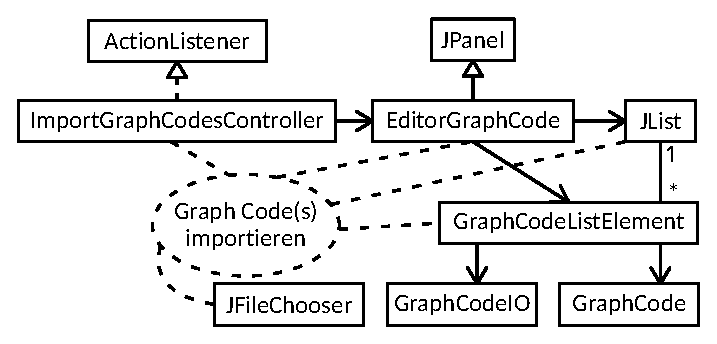
\includegraphics{chapter/chapter_3/mechanisms/mechanism-uc-1.1.eps}
    \caption{Mechanismus für den Anwendungsfall \hyperref[sec3:model:uc-1.1]{UC-1.1}.}
    \label{sec3:model:par:mechanism-use-cases:fig:mech-uc-1.1}
\end{figure}
\cref{sec3:model:par:mechanism-use-cases:fig:mech-uc-1.1} zeigt den Mechanismus für den Anwendungsfall \hyperref[sec3:model:uc-1.1]{UC-1.1}.
Sobald der Anwendungsfall \hyperref[sec3:model:uc-1.1]{UC-1.1} beginnt, benötigt es eine Komponente, die die in diesem Anwendungsfall enthaltenen Subaktionen steuert.
Diese Aufgabe übernimmt die Komponente \textit{ImportGraphCodesController}.
Da das Importieren von Graph Codes das Auswählen der jeweiligen Graph Code Datei(en) erfordert, benötigt es einen Auswahldialog \textit{JFileChooser}.
Die nun durch den Benutzer ausgewählten Dateien werden einer Liste in der Arbeitsfläche hinzugefügt.
Genauer ist diese Arbeitsfläche die linke Arbeitsfläche (siehe \cref{sec3:model:par:wireframe:fig:stage-1} \circitem{1}) und wird in diesem Diagramm durch \textit{EditorGraphCode} dargestellt.
Diese Arbeitsfläche zeigt eine (1) Liste \textit{JList} (siehe \cref{sec3:model:par:wireframe:fig:stage-2+3} \circitem{5}), welcher beliebig viele (*) Graph Codes \textit{GraphCodeListElement} hinzugefügt werden können.

\begin{figure}[htb]
    \centering
    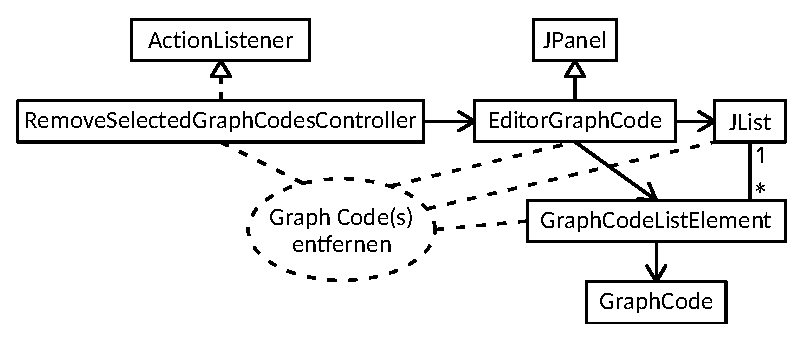
\includegraphics{chapter/chapter_3/mechanisms/mechanism-uc-1.2.eps}
    \caption{Mechanismus für den Anwendungsfall \hyperref[sec3:model:uc-1.2]{UC-1.2}.}
    \label{sec3:model:par:mechanism-use-cases:fig:mech-uc-1.2}
\end{figure}
\cref{sec3:model:par:mechanism-use-cases:fig:mech-uc-1.2} zeigt den Mechanismus für den Anwendungsfall \hyperref[sec3:model:uc-1.2]{UC-1.2}.
Der Mechanismus für den Anwendungsfall \hyperref[sec3:model:uc-1.2]{UC-1.2} ist sehr ähnlich im Vergleich zum Mechanismus für den Anwendungsfall \hyperref[sec3:model:uc-1.2]{UC-1.2}.
Einzig erwähnenswert ist die Komponente \textit{RemoveSelectedGraphCodesController}, die die notwendigen Subaktionen zum Entfernen von Graph Codes steuert.

\begin{figure}[htb]
    \centering
    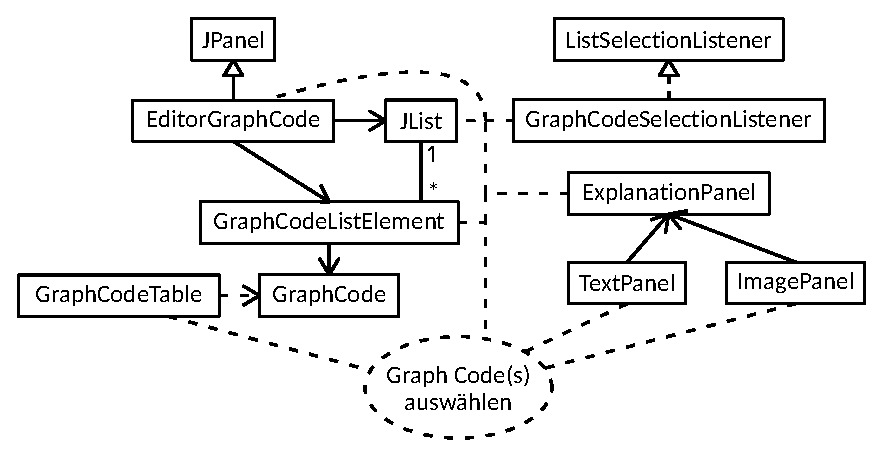
\includegraphics{chapter/chapter_3/mechanisms/mechanism-uc-1.3.eps}
    \caption{Mechanismus für den Anwendungsfall \hyperref[sec3:model:uc-1.3]{UC-1.3}.}
    \label{sec3:model:par:mechanism-use-cases:fig:mech-uc-1.3}
\end{figure}

\cref{sec3:model:par:mechanism-use-cases:fig:mech-uc-1.3} zeigt den Mechanismus für den Anwendungsfall \hyperref[sec3:model:uc-1.3]{UC-1.3}.
Der Anwendungsfall \hyperref[sec3:model:uc-1.3]{UC-1.3} beginnt mit der Auswahl von Graph Code(s).
Das Auswählen von Graph Codes beeinflusst mehrere Komponenten in der gesamten Benutzerschnittstelle.
Die Aktionen zur Einflussnahme auf diese Komponenten werden durch die Komponente \textit{GraphCodeSelectionListener} gesteuert.
Beeinflusste Komponenten umfassen die Komponente \textit{GraphCodeTable} (siehe \cref{sec3:model:par:wireframe:fig:stage-2+3} \circitem{6}), sowie die Komponente \textit{ExplanationPanel} (siehe \cref{sec3:model:par:wireframe:fig:stage-2+3} \circitem{2}), in der Benutzer zwischen Erklärungstypen umschalten können.
Die Komponenten \textit{ImagePanel} und \textit{TextPanel} sind die für die Erklärungstypen spezifischen Benutzerschnittstellen, und können durch \cref{sec3:model:par:wireframe:fig:stage-2+3} \circitem{7} umhergeschaltet werden.

% Mechanismus zu Anwendungsfall 1.5, und Mechanismus hier als Basis für die spätere Diskussion und den Aspekt der Operationsverkettung...
\begin{figure}[htb]
    \centering
    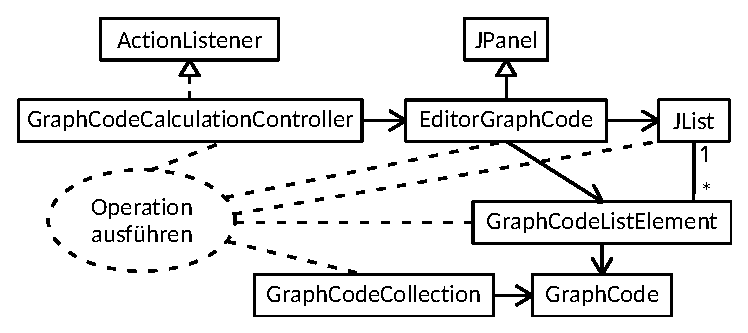
\includegraphics{chapter/chapter_3/mechanisms/mechanism-uc-1.5.eps}
    \caption{Mechanismus für den Anwendungsfall \hyperref[sec3:model:uc-1.5]{UC-1.5}.}
    \label{sec3:model:par:mechanism-use-cases:fig:mech-uc-1.5}
\end{figure}

\cref{sec3:model:par:mechanism-use-cases:fig:mech-uc-1.5} zeigt den Mechanismus für den Anwendungsfall \hyperref[sec3:model:uc-1.5]{UC-1.5}.
Der Anwendungsfall \hyperref[sec3:model:uc-1.5]{UC-1.5} \enquote{Operation ausführen} beginnt durch das Klicken des Knopfes \enquote{Execute}.
Die an diesem Anwendungsfall beteiligten Aktionen werden durch die Komponente \textit{GraphCodeCalculationController} gesteuert und geleitet.
Dies beinhaltet auch das Differenzieren der in Anwendungsfall \hyperref[sec3:model:uc-1.4]{UC-1.4} zuvor ausgewählten Operation.
Diese Operation kann die \textit{Vereinigung (Union)}, \textit{relative Differenz / Unterschied bzw. Subtraktion}, \textit{Gemeinsamkeiten (Similarities)} oder \textit{Unterschiede (Differences) }zwischen mehreren Graph Codes sein.
Besonders hierbei ist die \textit{Subtraktion}, die nur auf zwei Graph Codes angewandt werden kann.
Die Algorithmen zur Berechnung der Operationen der \textit{Vereinigung} von mehreren Graph Codes, sowie der \textit{Subtraktion} zweier Graph Codes werden bereits durch die Komponente \textit{GraphCodeCollection} bereitgestellt.
Im Folgenden werden Konzepte für die weiteren Operationen \textit{Gemeinsamkeiten} und \textit{Unterschiede} in Form von Pseudoalgorithmen vorgestellt, und es werden die an diesen Operationen beteiligten Komponenten, ihre Aufgaben, sowie durchzuführende Schritte beschrieben.

\begin{algorithm}[htb]
\caption{Berechne Gemeinsamkeiten}
\label{sec3:model:par:mechanism-use-cases:alg:sim}
\begin{algorithmic}[1]
\Require{Liste an Graph Codes: gcs}
\Ensure{Graph Code}
\Function{GetSimilarities}{$\text{gcs}$}
    %\State Graph Code für Gemeinsamkeiten (sim) $\gets$ new GraphCode
    %\State Vereinigung von Graph Codes (union) $\gets$ getUnion(gcs)
    %\State Vokabular von union (unionDic) $\gets$ new Vector(Vokabular von union)
    \State sim $\gets$ new GraphCode
    \State union $\gets$ getUnion(gcs)
    \State unionDic $\gets$ new Vector(union.getDictionary())
    \For{gc in gcs}
        \State \shortstack[l]{Entferne alle Elemente aus unionDic, \\die nicht im Vokabular von gc enthalten sind}
    \EndFor
    \State dictionary $\gets$ new Vector(unionDic)
    \State sim.setDictionary(dictionary)
    
    \For{gci in gcs}
        \For{s in dictionary}
            \For{t in dictionary}
                \State $\text{i} \gets \text{gci.getEdgeValueForTerms}(\text{s}, \text{t})$
                \State $\text{sim.setValueForTerms}(\text{s}, \text{t}, \text{i})$
            \EndFor
        \EndFor
    \EndFor
    \State \textbf{return} $\text{sim}$
\EndFunction
\end{algorithmic}
\end{algorithm}

\cref{sec3:model:par:mechanism-use-cases:alg:sim} zeigt einen Pseudoalgorithmus für die Operation \textit{Gemeinsamkeiten}.
Diese Algorithmus nimmt als Eingabe eine Liste an Graph Codes und gibt als Ergebnis einen Graph Code zurück.
Der Algorithmus kann in drei Bereiche unterteilt werden: \textit{Vorbereitung}, \textit{Berechnung} und \textit{Verwertung}.
Der Bereich \textit{Vorbereitung} umfasst die Zeilen 2 bis 4.
In diesem Bereich wird das Ergebnis als Objekt zum ersten Mal initialisiert.
Weiterhin wird die Vereinigung aller Graph Codes aus der Eingabe der Funktion mit der Funktion getUnion, welche durch die Komponente \textit{GraphCodeCollection} bereitgestellt wird, berechnet.
Ergebnis dieser Vereinigung ist wiederum ein Graph Code, dessen Vokabular zuletzt für die weitere Berechnung in den folgenden Bereichen aufbereitet wird.
Der zweite Bereich \textit{Berechnung} umfasst die Zeilen 5 bis 6.
In diesem Bereich wird das Vokabular der Vereinigung (unionDic) mit dem Vokabular aller Graph Codes aus der Eingabe miteinander verglichen und es werden alle Merkmale aus unionDic, die nicht in irgendeinem Vokabular eines Graph Codes aus der Eingabe vorkommen, entfernt.
Übrig bleiben die Merkmale, die in jedem Graph Code aus der Eingabe vorkommen.
Der dritte Bereich \textit{Verwertung} umfasst die übrigen Zeilen 7 bis 14.
Dem Objekte sim, welches das Ergebnis repräsentiert, wird das Vokabular unionDic gesetzt.
Im weiteren Verlauf wird für jeden Graph Code zeilen- und spaltenweise der Wert für ein Paar aus Merkmalen in der Adjanzenzmatrix bestimmt und dieser Wert in der Matrix des Ergebnisses eingetragen.
Schlussendlich wird das Ergebnis als Ausgabe zurückgegeben.
% comment-soigner u. csm katze allein lassen
In \cref{sec3:model:par:mechanism-use-cases:fig:gc1-2-similarities} wird die beispielhafte Berechnung der Gemeinsamkeiten zweier Graph Codes dargestellt.

\begin{figure}[!ht]
  \centering
  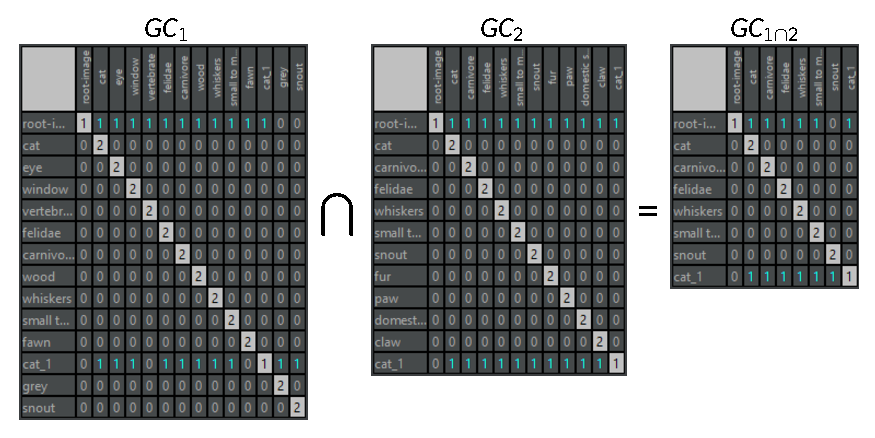
\includegraphics{chapter/chapter_3/algorithms/gc1-2-similarities-ex}
  \caption{Beispielhafte Visualisierung für die Berechnung der Gemeinsamkeiten zweier Graph Codes $GC_1$ und $GC_2$.}
  \label{sec3:model:par:mechanism-use-cases:fig:gc1-2-similarities}
\end{figure}

\begin{algorithm}[htb]
\caption{Berechne Unterschiede}
\label{sec3:model:par:mechanism-use-cases:alg:dif}
\begin{algorithmic}[1]
\Function{GetDifferences}{$\text{gcs}$}
    %\State Graph Code für Gemeinsamkeiten (sim) $\gets$ new GraphCode
    %\State Vereinigung von Graph Codes (union) $\gets$ getUnion(gcs)
    %\State Vokabular von union (unionDic) $\gets$ new Vector(Vokabular von union)
    \State diff $\gets$ new GraphCode
    \State union $\gets$ getUnion(gcs)
    \State unionDic $\gets$ new Vector(union.getDictionary())
    \For{gc in gcs}
        \State \shortstack[l]{Entferne alle Elemente aus unionDic, \\die nicht im Vokabular von gc enthalten sind}
    \EndFor
    
    \State \shortstack[l]{Alle Merkmale bestimmen, die im Vokabular der Vereinigung union,\\ aber nicht im Vokabular unionDic enthalten sind.}
    \State dictionary $\gets$ new Vector(unionDic)
    \State diff.setDictionary(dictionary)
    
    \For{gci in gcs}
        \For{s in dictionary}
            \For{t in dictionary}
                \State $\text{i} \gets \text{gci.getEdgeValueForTerms}(\text{s}, \text{t})$
                \State $\text{diff.setValueForTerms}(\text{s}, \text{t}, \text{i})$
            \EndFor
        \EndFor
    \EndFor
    \State \textbf{return} $\text{diff}$
\EndFunction
\end{algorithmic}
\end{algorithm}

\cref{sec3:model:par:mechanism-use-cases:alg:dif} zeigt einen Pseudoalgorithmus für die Operation \textit{Unterschiede}.
Dieser Algorithmus ist sehr ähnlich zum \cref{sec3:model:par:mechanism-use-cases:alg:sim} und nimmt ebenfalls eine Liste an Graph Codes und gibt als Ergebnis einen Graph Code zurück.
Zudem kann dieser Algorithmus ebenfalls in die gleichen Bereiche unterteilt werden.
Mehr noch sind die Bereiche \textit{Vorbereitung} (Zeile 2 bis 4) und \textit{Verwertung} (Zeile 10 bis 15) identisch und Unterschiede in den Algorithmen bestehen nur im Bereich \textit{Berechnung} (Zeile 6 - 7).
Genauer besteht der einzige Unterschied im Vergleich zum \cref{sec3:model:par:mechanism-use-cases:alg:sim}, dass unterschiedliche Merkmale in mehreren Graph Codes das Gegenteil der gemeinsamen Merkmale in mehreren Graph Codes ist.
In \cref{sec3:model:par:mechanism-use-cases:fig:gc1-2-differences} wird die beispielhafte Berechnung der Unterschiede zweier Graph Codes dargestellt.

\begin{figure}[!ht]
  \centering
  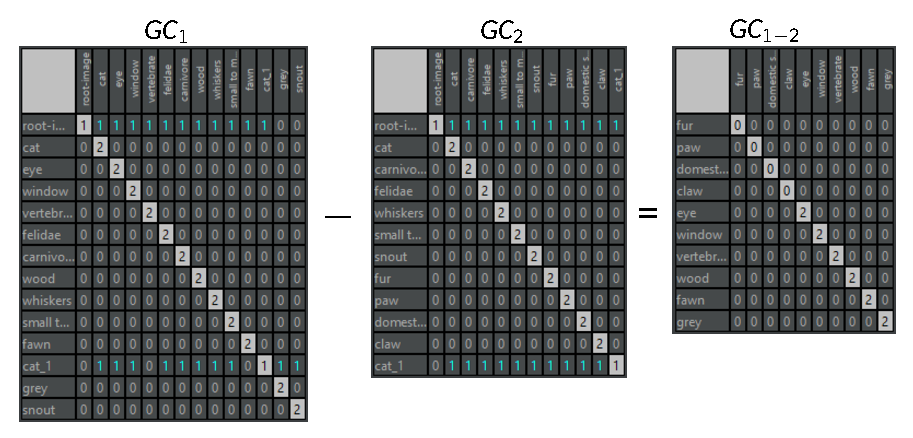
\includegraphics{chapter/chapter_3/algorithms/gc1-2-differences-ex}
  \caption{Beispielhafte Visualisierung für die Berechnung der symmetrische Differenz bzw. Unterschiede zweier Graph Codes $GC_1$ und $GC_2$.}
  \label{sec3:model:par:mechanism-use-cases:fig:gc1-2-differences}
\end{figure}

Zusammengefasst und einfacher ausgedrückt wird in der Operation \textit{Gemeinsamkeiten} die Schnittmenge aller Vokabulare von Graph Codes, welche wiederum nur Mengen von Merkmalen sind, gebildet.
Analog wird in der Operation \textit{Unterschiede} die symmetrische Differenz aller Vokabular von Graph Codes gebildet, welches dem Gegenteil der Schnittmenge aller Vokabulare von Graph Codes entspricht.
Dies unterscheidet die Operation \textit{Unterschiede} von der durch die Komponente \textit{GraphCodeCollection} bereitgestellten Operation \textit{Subtraktion}, welche nur die relative Differenz zweier Graph Codes bildet.

\FloatBarrier

\paragraph{Sequenzdiagramme}
\label{sec3:model:par:seq-use-cases}
Sequenzdiagramme modellieren den konkreten zeitlichen Verlauf von mitunter komplexen Operationen in einem Klassenmodell unter Einbeziehung der in diesen Operationen beteiligten Objekten.
Die in einer Operation beteiligten Objekte werden dabei am oberen Rand des Diagramms als ein Rechteck mit einer gestrichelten vertikalen Linie dargestellt.
Diese gestrichelte vertikale Linie wird als \textit{Lebenslinie} bezeichnet und symbolisiert die Lebenszeit eines Objektes, welche von oben nach unter voranschreitet.
Interaktionen zwischen Objekten, wie z.B. dem Aufrufen einer Operation eines Objektes durch ein anderes Objekt, geschehen durch das Senden von Nachrichten zwischen diesen.
Die gängigsten Formen von Nachrichten sind:

\begin{figure}[htb]
    \centering
    \begin{subfigure}{.25\textwidth}
        \centering
        \tikz{
            \begin{umlseqdiag}
                \umlobject[x=0,fill=white]{A}
                \umlobject[x=1,fill=white]{B}

                \begin{umlcall}{A}{B}
                \end{umlcall}
            \end{umlseqdiag}
        }
        \caption{}
        \label{sec3:model:par:seq-use-cases:subfig:sync-message}
    \end{subfigure}%
    \begin{subfigure}{.25\textwidth}
        \centering
        \tikz{
            \begin{umlseqdiag}
                \umlobject[x=0,fill=white]{A}
                \umlobject[x=1,fill=white]{B}

                \begin{umlcall}[type=asynchron]{A}{B}
                \end{umlcall}
            \end{umlseqdiag}
        }
        \caption{}
        \label{sec3:model:par:seq-use-cases:subfig:async-message}
    \end{subfigure}%
    \begin{subfigure}{.25\textwidth}
        \centering
        \tikz{
            \begin{umlseqdiag}
                \umlobject[x=0,fill=white]{A}
                \umlobject[x=3,fill=white]{B}

                \begin{umlcall}[op={Nachricht},return={Antwort}]{A}{B}
                \end{umlcall}
            \end{umlseqdiag}
        }
        \caption{}
        \label{sec3:model:par:seq-use-cases:subfig:return-message}
    \end{subfigure}%
    \begin{subfigure}{.25\textwidth}
        \centering
        \tikz{
            \begin{umlseqdiag}
                \umlobject[fill=white]{A}

                \begin{umlcallself}{A}
                \end{umlcallself}
            \end{umlseqdiag}
        }
        \caption{}
        \label{sec3:model:par:seq-use-cases:subfig:selfcall}
    \end{subfigure}
    \caption{(i) Synchrone Nachricht, (ii) Asynchrone Nachricht, (iii) Antwort auf Nachricht, (iv) Selbstdelegation / Selbstaufruf.}
    \label{fig:test}
\end{figure}

\begin{enumerate}[label=(\roman{enumi})]
    \item \textit{Synchrone Nachrichten} werden durch einen geschlossenen, gefüllten Pfeil \tikz{ \draw[-{Triangle[angle=90:5pt,length=4mm,fill=black]}] (0,0) -- (0.7,0) {}; } dargestellt.
    Eine synchrone Nachricht repräsentiert einen direkten Aufruf einer Operation vom Dienstnutzenden (Sender) zum Dienstleistenden (Empfänger).
    Eine wichtige Eigenschaft, die diesem Nachrichtentyp seinen Namen verleiht ist, dass der Sender auf die Antwort seiner Nachricht wartet, bevor er weitere Nachrichten sendet.
    \item \textit{Asynchrone Nachricht} werden durch einen offenen, spitzen Pfeil \tikz[baseline=-.6ex]{ \draw[-{angle 45}] (0,0) -- (0.7,0) {}; } dargestellt.
    Im Gegensatz zu einer synchronen Nachricht wartet der Sender nach Senden der Nachricht nicht mehr auf eine Antwort des Empfängers, sondern kann unmittelbar weitere Nachrichten senden.
    Folglich sind bei dieser Art von Nachricht die Sender und Empfänger nicht mehr synchron zueinander.
    \item Eine Nachricht vom Typ \textit{Antwort} ist eine Antwort auf eine asynchrone Nachricht und wird durch einen gestrichelten, entgegengesetzten Pfeil \tikz[baseline=-0.6ex]{ \draw[{angle 45}-, dashed] (0,0) -- (0.7,0){};} dargestellt.
    Eine Antwort führt den Kontrollfluss zurück auf den Sender der Nachricht nachdem die Operation vom Empfänger abgeschlossen wurde.
    \item \textit{Selbstdelegation} / \textit{Selbstaufruf} ist eine Nachricht eines Objektes auf sich selbst und tritt meist bei rekursiven Methoden auf.
\end{enumerate}

Im Folgenden werden für ausgewählte Anwendungsfälle Sequenzdiagramme vorgestellt und beschrieben.

\begin{figure}[htb]
    \centering
    \resizebox{\textwidth}{!}{
        \begin{tikzpicture}
            \begin{umlseqdiag}
                % Actors
                \umlactor[fill=white, scale=0.7]{Benutzer}
                
                % Objects
                \umlobject[x=0, fill=white]{Benutzer}
                \umlmlobject[x=3.3, fill=white]{sgc}{\shortstack[c]{Select\\GraphCodes\\Controller}}
                \umlobject[x=6, fill=white]{JFileChooser}
                \umlmlobject[x=9, fill=white]{egc}{\shortstack[c]{Editor\\GraphCode}}
                \umlmlobject[x=12, fill=white]{gcle}{\shortstack[c]{GraphCode\\ListElement}}
                \umlmlobject[x=15, fill=white]{gcio}{GraphCodeIO}

                % Calls
                \begin{umlcall}[padding=-1pt,dt=6.5,op={\shortstack[c]{Select \\ Graph Codes}}]{Benutzer}{sgc}
                    \begin{umlcall}[op={zeige Dialog}, return={Zustand}]{sgc}{JFileChooser}
                    \end{umlcall}
                    \begin{umlcall}[dt=4,op={Gib Liste}, return={Liste}]{sgc}{egc}
                    \end{umlcall}
                    \begin{umlfragment}[type=if, label={\shortstack[c]{Zustand \\ \textit{öffnen}}}]
                        \begin{umlcall}[padding=2.5pt,dt=5, op={\shortstack[c]{Ausgewählte \\ Datei(en)}}, return={Datei(en)}]{sgc}{JFileChooser}
                        \end{umlcall}
                        \begin{umlfragment}[type=for (files)]
                            \begin{umlcall}[padding=2.5, op={Erzeuge aus Datei}, return={GraphCodeListElement (gcle)}]{sgc}{gcle}
                                \begin{umlcall}[padding=2.5pt,op={\shortstack[c]{Graph Code \\ Datei lesen}}, return={Graph Code}]{gcle}{gcio}
                                \end{umlcall}
                            \end{umlcall}
                            \begin{umlcall}[op={gcle der Liste hzf.}]{sgc}{egc}
                            \end{umlcall}
                        \end{umlfragment}
                    \end{umlfragment}
                \end{umlcall}
            \end{umlseqdiag}
        \end{tikzpicture}
    }
    \caption{Sequenzdiagramm für den Anwendungsfall \hyperref[sec3:model:uc-1.1]{UC-1.1}.}
    \label{sec3:model:par:seq-use-cases:fig:seq-diag-uc-1.1}
\end{figure}

\cref{sec3:model:par:seq-use-cases:fig:seq-diag-uc-1.1} zeigt ein Sequenzdiagramm für den Anwendungsfall \hyperref[sec3:model:uc-1.1]{UC-1.1}.
Es zeigt, wie der Benutzer die Aktion \enquote{Graph Code(s) importieren} durch einen Klick auf den Knopf \enquote{Select Graph Code(s)} initiiert.
Weitere Aktionen werden dann von der Komponente \textit{SelectGraphCodesController} durchgeführt.
Diese Aktionen umfassen das Anzeigen eines Dateiauswahldialogs und der in diesem Dialog ausgewählten Dateien.
Für alle ausgewählte Dateien \textit{for (files)} werden dann Listenelemente erzeugt, die der Liste hinzugefügt werden können.
Hierfür müssen die Graph Code Dateien durch die Komponente \textit{GraphCodeIO} eingelesen und in ein Objekt umgewandelt werden.

\begin{figure}[!ht]
    \centering
    \begin{tikzpicture}
            \begin{umlseqdiag}
                % Actors
                \umlactor[fill=white, scale=0.7]{Benutzer}

                % Objects
                \umlobject[x=0, fill=white]{Benutzer}
                \umlmlobject[x=3.3, fill=white]{rsgc}{\shortstack[c]{Remove\\Selected\\GraphCodes\\Controller}}
                \umlmlobject[x=6, fill=white]{egc}{\shortstack[c]{Editor\\GraphCode}}
                \umlobject[x=8, fill=white]{JList}

                % Calls
                \begin{umlcall}[padding=-2,dt=6.5,op={\shortstack[c]{Remove Selected \\ Graph Codes}}]{Benutzer}{rsgc}
                    \begin{umlcall}[dt=4,op={Gib Liste}, return={Liste}]{rsgc}{egc}
                    \end{umlcall}
                    \begin{umlcall}[dt=6,op={\shortstack[c]{Ausgewählte \\Elemente}}, return={Indizes i der Elemente}]{rsgc}{JList}
                    \end{umlcall}
                    \begin{umlfragment}[type=for(ind : i)]
                        \begin{umlcall}[dt=5,op={\shortstack[c]{Entferne Element \\ an Pos. ind}}]{rsgc}{JList}
                        \end{umlcall}
                    \end{umlfragment}
                \end{umlcall}
            \end{umlseqdiag}
        \end{tikzpicture}
    \caption{Sequenzdiagramm für den Anwendungsfall \hyperref[sec3:model:uc-1.2]{UC-1.2}.}
    \label{sec3:model:par:seq-use-cases:fig:seq-diag-uc-1.2}
\end{figure}


\cref{sec3:model:par:seq-use-cases:fig:seq-diag-uc-1.2} zeigt ein Sequenzdiagramm für den Anwendungsfall \hyperref[sec3:model:uc-1.2]{UC-1.2}.
Es zeigt, wie der Benutzer die Aktion \enquote{Graph Code(s) entfernen} durch einen Klick auf den Knopf \enquote{Remove selected Graph Code(s)} initiiert.
Weitere Aktionen werden dann von der Komponente \textit{RemoveSelectedGraphCodesController} durchgeführt.
Diese Aktionen umfassen die Abfrage der ausgewählten Elemente in der Liste und die Rückführung der Indizes, die die Positionen dieser Elemente wiedergeben.
Anhand dieser Indizes kann der Liste mitgeteilt werden das Element an der Position eines Indexes zu entfernen.

\begin{figure}[!ht]
    \centering
    \resizebox{\textwidth}{!}{
        \begin{tikzpicture}
            \begin{umlseqdiag}
                % Actors
                \umlactor[fill=white, scale=0.7]{Benutzer}

                % Objects
                \umlobject[x=0, fill=white]{Benutzer}
                \umlmlobject[x=3.3, fill=white]{gcs}{\shortstack[c]{Graph Code \\ SelectionListener}}
                \umlmlobject[x=8, fill=white]{egc}{\shortstack[c]{Editor\\GraphCode}}
                \umlobject[x=10, fill=white]{JList}
                \umlmlobject[x=12, fill=white]{gct}{\shortstack[c]{GraphCode \\ Table}}
                \umlmlobject[x=14.5, fill=white]{ep}{\shortstack[c]{Explanation \\ Panel}}

                % Calls
                \begin{umlcall}[padding=0,dt=6.5,op={\shortstack[c]{Graph Code \\ Selection}}]{Benutzer}{gcs}
                    \begin{umlcall}[op={Gib Liste}, return={Liste}]{gcs}{egc}
                    \end{umlcall}
                    \begin{umlcall}[padding=2.5,dt=4,op={\shortstack[c]{Gib ausgewähltes Element}}, return={\shortstack[c]{GraphCodeListElement (gcle)}}]{gcs}{JList}
                    \end{umlcall}
                    \begin{umlcall}[padding=2.5,dt=5,op={\shortstack[c]{Gib \\GraphCodeTable}}, return={\shortstack[c]{GraphCodeTable}}]{gcs}{egc}
                    \end{umlcall}
                    \begin{umlcall}[dt=4,op={Setze Graph Code}]{gcs}{gct}
                    \end{umlcall}
                    \begin{umlcall}[padding=2.5,op={\shortstack[c]{Gib \\ ExplanationPanel}}, return={ExplanationPanel}]{gcs}{egc}
                    \end{umlcall}
                    \begin{umlcall}[dt=4,op={Setze Graph Code}]{gcs}{ep}
                    \end{umlcall}
                \end{umlcall}
            \end{umlseqdiag}
        \end{tikzpicture}
    }
    \caption{UML-Sequenzdiagramm für den Anwendungsfall \hyperref[sec3:model:uc-1.3]{UC-1.3}.}
    \label{sec3:model:par:seq-use-cases:fig:seq-diag-uc-1.3}
\end{figure}


\cref{sec3:model:par:seq-use-cases:fig:seq-diag-uc-1.3} zeigt ein Sequenzdiagramm für den Anwendungsfall \hyperref[sec3:model:uc-1.3]{UC-1.3}.
Es zeigt, wie der Benutzer die Aktion \enquote{Graph Code(s) auswählen} durch eine Auswahl auf ein Element in der Liste initiiert.
Die Ausführungen der weiteren Aktionen werden dann von der Komponente \textit{GraphCodeSelectionListener} übernommen.
Zusammengefasst wird hier das aktuell ausgewählte Element in der Liste abgefragt und von der Liste zurückgeführt.
Dieses Komponente \textit{GraphCodeListElement} enthält wiederum die Komponente \textit{GraphCode}, welche dann anderen Schnittstellen, wie der Komponente \textit{GraphCodeTable} oder \textit{ExplanationPanel} zur weiteren Verarbeitung mitgeteilt werden kann.
Die Komponente \textit{ExplanationPanel} stellt wiederum die Komponenten \textit{ImagePanel} und \textit{TextPanel} zur Verfügugn bzw. hält diese Komponenten inne.
Die weitere Verarbeitung eines Graph Codes erfolgt dann analog durch diese Komponenten.

\begin{figure}[!ht]
    \centering
    \resizebox{\textwidth}{!}{
        \begin{tikzpicture}
            \begin{umlseqdiag}
                % Actors
                \umlactor[fill=white, scale=0.7]{Benutzer}

                % Objects
                \umlobject[x=0, fill=white]{Benutzer}
                \umlmlobject[x=3.3, fill=white]{gcs}{\shortstack[c]{Graph Code \\ Calculation \\ Controller}}
                \umlmlobject[x=8, fill=white]{egc}{\shortstack[c]{Editor\\GraphCode}}
                \umlobject[x=10, fill=white]{JList}
                \umlmlobject[x=12, fill=white]{gc}{\shortstack[c]{GraphCode\\Collection}}
                \umlmlobject[x=15, fill=white]{gcle}{\shortstack[c]{GraphCode\\ListElement}}

                % Calls
                \begin{umlcall}[padding=0,dt=4,op={\shortstack[c]{Execute}}]{Benutzer}{gcs}
                    \begin{umlcall}[op={Gib Liste}, return={Liste}]{gcs}{egc}
                    \end{umlcall}
                    \begin{umlcall}[padding=2.5,dt=4,op={\shortstack[c]{Gib ausgewählte Elemente}}, return={\shortstack[c]{GraphCodeListElement(e) (gcle)}}]{gcs}{JList}
                    \end{umlcall}
                    \begin{umlcall}[op={Gib Aktion}, return={Aktion}]{gcs}{egc}
                    \end{umlcall}
                    \begin{umlfragment}[inner xsep=5,type=switch, label={union}]
                        \begin{umlcall}[padding=2.5,op={Berechne Vereinigung von gcle's}, return={Graph Code}]{gcs}{gc}
                        \end{umlcall}
                        \umlfpart[subtract]
                        \begin{umlcall}[padding=2.5,op={Berechne Subtraktion von gcle's}, return={Graph Code}]{gcs}{gc}
                        \end{umlcall}
                        \umlfpart[similarity]
                        \begin{umlcall}[padding=2.5,op={Berechne Gemeinsamkeiten von gcle's}, return={Graph Code}]{gcs}{gc}
                        \end{umlcall}
                        \umlfpart[differences]
                        \begin{umlcall}[padding=2.5,op={Berechne Unterschiede von gcle's}, return={Graph Code}]{gcs}{gc}
                        \end{umlcall}
                    \end{umlfragment}
                    \begin{umlcall}[padding=2.5, dt=-1,op={Erzeuge aus Graph Code}, return={GraphCodeListElement (glce)}]{gcs}{gcle}
                    \end{umlcall}
                    \begin{umlcall}[dt=1,op={Füge gcle Liste hinzu}]{gcs}{JList}
                    \end{umlcall}
                \end{umlcall}
            \end{umlseqdiag}
        \end{tikzpicture}
    }
    \caption{UML-Sequenzdiagramm für den Anwendungsfall \hyperref[sec3:model:uc-1.5]{UC-1.5}.}
    \label{sec3:model:par:seq-use-cases:fig:seq-diag-uc-1.5}
\end{figure}


\cref{sec3:model:par:seq-use-cases:fig:seq-diag-uc-1.5} zeigt ein Sequenzdiagramm für den Anwendungsfall \hyperref[sec3:model:uc-1.5]{UC-1.5}.
Es zeigt, wie der Benutzer die Aktion \enquote{Operation ausführen} durch einen Klick auf den Knopf \enquote{Execute} initiiert.
Die weiteren Aktionen werden dann von der Komponenten \textit{GraphCodeCalculationController} übernommen.
Diese Aktionen umfassen die Abfrage der ausgewählten Elemente aus der Liste und die Rückführung dieser Elemente, damit die in diesen Elementen gespeicherten Graph Codes im weiteren Verlauf verarbeitet werden können.
Die Verarbeitung ist dabei abhängig von der in Anwendungsfall \hyperref[sec3:model:uc-1.4]{UC-1.4} ausgewählten Operation.
Die Differenzierung dieser Aktionen wird im Sequenzdiagramm durch die Box \textit{switch} dargestellt.
Schlussendlich wird mit dem Ergebnis ein neues Element für die Liste erzeugt und der Liste hinzugefügt.

\FloatBarrier

\subsubsection{Diskussion}
\label{sec3:model:subsubsec:fz1:discussion}
In diesem Abschnitt wurden die offenen Herausforderungen \hyperref[sec2:sota:oi:1.1]{\textbf{OH 1.1}} und \hyperref[sec2:sota:oi:1.1]{\textbf{OH 1.2}} adressiert.
In \cref{sec3:model:subsubsec:explainability-through-genai} wurde die offene Herausforderung \hyperref[sec2:sota:oi:1.1]{\textbf{OH 1.1}} behandelt und Möglichkeiten vorgestellt, wie durch generative KI Erklärbarkeit erreicht werden kann.
In \cref{sec3:model:subsubsec:use-cases} wurde die offene Herausforderung \hyperref[sec2:sota:oi:1.2]{\textbf{OH 1.2}} behandelt und es wurden Anwendungsfälle aus der Perspektive von Benutzern des GMAF identifiziert und beschrieben.
Darüber hinaus wurden Wireframes für eine Benutzerschnittstelle mit geeigneten Interaktionsmöglichkeiten für den sinnvollen Einsatz von Systemen generativer KI zur Erklärung von Graph Codes konzipiert und weiter ausgeführt.
Weiterhin wurden anhand der identifizierten Anwendungsfälle und den dazu entsprechenden textuellen Beschreibungen Mechanismen erstellt, um die an den Anwendungsfällen beteiligten Komponenten zu identifizieren.
Anhand der Anwendungsfälle und der mit diesen Mechanismen identifizierten Komponenten konnten daraufhin Sequenzdiagramme zur genaueren Ablaufbeschreibung erstellt werden.

Die in diesem Abschnitt gewonnen Erkenntnisse bieten die Grundlage zur Entwicklung einer geeignete Benutzerschnittstelle zur Erklärbarkeit von Graph Codes mittels generativer KI.

\clearpage

\subsection{FZ 2.2/TB Integration generativer KI in das GMAF}
\label{sec3:model:subsec:fz-integration}
Dieser Abschnitt befasst sich mit der Modellierung der \enquote{Integration generativer KI in das GMAF}. Dabei werden die in FZ 2.1/O identifizierten, offenen Herausforderungen \hyperref[sec2:sota:oi:2.1]{\textbf{OH 2.1}} und \hyperref[sec2:sota:oi:2.2]{\textbf{OH 2.2}} adressiert.
Ziel dieses Abschnitts ist es Konzepte für die Überführung von Graph Codes in eine geeignete Form zur Eingabe in ein System generativer KI zu entwickeln, sowie Konzepte für die Integration generativer KI zu entwickeln.
Hierzu wird in \cref{sec3:model:subsubsec:gc-transformation} die offene Herausforderung \hyperref[sec2:sota:oi:2.1]{\textbf{OH 2.1}} und in \cref{sec3:model:subsubsec:genai-integration} die offene Herausforderung \hyperref[sec2:sota:oi:2.2]{\textbf{OH 2.2}} adressiert.

\subsubsection{Transformation von Graph Codes}
\label{sec3:model:subsubsec:gc-transformation}
Dieser Abschnitt widmet sich der Entwicklung von Konzepten zur Überführung der in Graph Codes gespeicherten Informationen, sowie der mit Graph Codes assoziierten Informationen in eine geeignete Form, die als Eingabe in ein System generativer KI verwendet werden kann.
Wie bereits in \cref{sec2:sota} recherchiert wurde, erfolgt die Eingabe in ein System generativer KI durch eine Eingabeaufforderung bzw. Prompt, die im Endeffekt eine beliebig lange Zeichenkette sein kann.
Die geeignete Form, in die es also Graph Codes zu Überführen gilt, sind somit Prompts.
Bevor allerdings mit dem eigentlichen Konzipieren der Transformation von Graph Codes in Prompts begonnen werden kann, ist es sinnvoll zu bestimmen, welche Informationen im Rahmen von Graph Codes überhaupt für eine Erklärung relevant sein können.
Von besonderer Relevanz für eine Erklärung sind in erster Linie die Merkmale bzw. das Vokabular, gespeichert im Wörterbuch eines Graph Codes, sowie die Informationen über bestehende Beziehungen zwischen diesen Merkmalen, gespeichert in einer zweidimensionalen, quadratischen Matrix.
Daher werden in diesem Abschnitt erst Konzepte für die Grundlagen von Graph Codes entwickelt.
Im Anschluss werden dann Konzepte für die mit Graph Codes assoziierten Informationen besprochen.
Die in den folgenden Abschnitten genannten Beispiele werden auf dem in \cref{sec3:model:subsubsec:gc-transformation:tab:gc-trans-ex} dargestellten Graph Code basieren.
% Beispiel eines Graph Codes für die Transformation (nur Matrix).

\begin{table}[htb]
  \begin{tabular}{rcccccc}
    &  \begin{turn}{90}root-image\end{turn}
    & \begin{turn}{90}cloud\end{turn}
    & \begin{turn}{90}water\end{turn}
    & \begin{turn}{90}sky\end{turn}
    & \begin{turn}{90}lake\end{turn}
    & \begin{turn}{90}dusk\end{turn} \\
    \hline

    root-image   & 1 & 1 & 1 & 1 & 1 & 1 \\
    cloud        & 0 & 2 & 0 & 3 & 0 & 0 \\
    water        & 0 & 0 & 2 & 0 & 3 & 0 \\
    sky          & 0 & 0 & 0 & 2 & 0 & 0 \\
    lake         & 0 & 0 & 4 & 0 & 2 & 0 \\
    dusk         & 0 & 0 & 0 & 0 & 0 & 2
  \end{tabular}
  \caption{Graph Code zum Beispiel der folgenden Transformationen.}
  \label{sec3:model:subsubsec:gc-transformation:tab:gc-trans-ex}
\end{table}

\paragraph{Transformation des Vokabulars}
Das Vokabular eines Graph Codes ist eine Menge aus Merkmalen, welche wiederum beliebig lange Zeichenketten sein können.
Eine einfache Art das Vokabular eines Graph Codes in eine Prompt zu überführen, ist somit einfach die Merkmale in Textform aufzuzählen.
Zusätzlich wird dem System durch eine in der Prompt vorangestellte Instruktion erklärt, welche Bedeutung die Elemente in der Aufzählung besitzen.
Ein entsprechendes Beispiel nach \cref{sec3:model:subsubsec:gc-transformation:tab:gc-trans-ex} hierfür wäre folgende Prompt: \enquote{The elements in the following list represent feature vocabulary terms and describe features extracted from multimedia files: root-image, cloud, water, sky, lake, dusk}.
Eine solche Transformation des Vokabulars wird durch die Komponente \textit{GraphCode} ermöglicht und kann in der entsprechenden Komponente des Erklärungstyps \textit{ImagePanel} oder \textit{TextPanel} durch eine Funktion \textit{setUpPrompt} eingesetzt werden.
\cref{sec3:model:subsubsec:gc-transformation:fig:set-up-prompt} zeigt ein einfaches Klassendiagramm mit den Komponenten \textit{ImagePanel}, \textit{TextPanel} und der Funktion \textit{setUpPrompt}.

\begin{figure}[htb]
    \centering
    \begin{tikzpicture}[assocstyle/.style={-{Straight Barb[angle'=60,scale=4]}}]
        \umlsimpleclass{ExplanationPanel}

        \umlclass[below left=4mm and -3mm of ExplanationPanel]{ImagePanel}{}{
            - setUpPrompt() : String \\
        }
        \umlclass[below right=4mm and -3mm of ExplanationPanel]{TextPanel}{}{
            - setUpPrompt() : String \\
        }

        \umluniassoc[assocstyle]{ImagePanel}{ExplanationPanel}
        \umluniassoc[assocstyle]{TextPanel}{ExplanationPanel}
    \end{tikzpicture}
    \caption{Einfaches Klassendiagramm für die Erklärungspaneele.}
    \label{sec3:model:subsubsec:gc-transformation:fig:set-up-prompt}
\end{figure}

% Erst Transformation vom Vokabular...
% Wie könnte das Vokabular transfomiert werden?
% Beispiele für solch eine Transformation (nur konzeptuelle Instruktionen (Prompting))
% Wo würde so eine Transformation umgesetzt werden?

\paragraph{Transformation der Matrix}
Die Adjazenzmatrix eines Graph Codes ist eine zweidimensionale, quadratische Matrix, dessen Anzahl an Zeilen bzw. Spalten äquivalent zur Größe des Vokabulars ist.
Die Werte der Einträge in der Matrix geben Aufschluss über das Vorhandensein von Beziehungen, sowie über die Bedeutung bzw. Art der Beziehung.
Bei der Transformation der Matrix müssen daher zwei Aspekte berücksichtigt werden: Das allgemeine Überführen der Informationen aus der Matrix, sowie das Überführen der Werte bzw. der Kodierung der Beziehungen und ihren Bedeutungen.

Eine einfache und naive Transformation kann bereits durch die Funktion \textit{toString} erfolgen, die durch die Komponente \textit{GraphCode} bereitgestellt wird.
Diese Funktion überführt die Informationen eines Graph Codes in das JSON-Format.
Ein Beispiel für so ein JSON-Format kann in \cref{sec2:sota:subsec:fz2:lst:gc-ex-json} eingesehen werden.
Die Tatsache, dass die GPT-Modelle in der Lage sind dieses Format zu analysieren und zu verarbeiten, begünstigt diese Herangehensweise.
Ein Beispiel nach \cref{sec3:model:subsubsec:gc-transformation:tab:gc-trans-ex} hierfür kann folgende Prompt sein: \enquote{The following JSON string represents a matrix. The matrix is a square twodimensional matrix where each element represents the relationship between two words: \{"matrix":\newline[[1,1,1,1,1,1],[0,2,0,0,0,0],[0,0,2,0,0,0],[0,0,0,2,0,0],[0,0,0,0,2,0],[0,0,0,0,0,2]]\}}.

Die Umsetzung dieser Transformation findet in der Funktion \textit{toString} in der Komponente \textit{GraphCode} statt und kann in der entsprechenden Komponente des Erklärungstypes \textit{ImagePanel} oder \textit{TextPanel} in der Funktion \textit{setUpPrompt} eingesetzt werden.

Ein Nachteil an dieser Herangehensweise ist das Verhältnis zum Platzverbrauch im Zeichenformat.
Aufgrund der quadratischen Natur der Adjazenzmatrix wird überproportional viel Platz verbraucht, was inbesondere anhand des immer weiter steigenden Detaillierungsgrades (LOD) als problematisch betrachtet werden muss.
Dies führt auch zu einem zunehmenden Tokenverbrauch, was in Bezug auf einige Modelle, wie z.B. Dall-E 2, die Zeichen- bzw. Tokenbeschränkungen besitzen, ebenfalls ein Problem darstellen könnte.
Eine Möglichkeit diesem Problem zu begegnen, wäre durch das Prüfen der Tokenlänge in der entstandenen Prompt.
Das Werkzeug \textit{Tokenizer}, vorgestellt in \cref{sec2:sota:par:tokenizer}, kann hierfür beim Zusammensetzen der Prompt verwendet werden.
Da hierdurch das Problem zwar erkannt, allerdings nicht gelöst wird, wird im Folgenden eine verbesserte Herangehensweise zum Transformieren der Informationen eines Graph Codes vorgestellt.

Die verbesserte Herangehensweise zur Überführung der Informationen eines Graph Codes reduziert die zu transformierenden Informationen auf ein Minimum.
Anders ausgedrückt, werden in dieser Herangehensweise nur die Informationen betrachtet und transformiert, die von Interesse sind.
Dies sind insbesondere die Einträge in einer Matrix, die überhaupt über eine Beziehung verfügen, ungeachtet der Kodierung bzw. des Typs der Beziehung.
Da jedes Merkmal $n$ Beziehungen zu anderen Merkmalen aufweisen kann, könnte sich das Format $<i_{t}> - <i_{t_{1}},...,i_{t_{n}}>$ gut zur Darstellung von Beziehungen zwischen Merkmalen eignen.
Der Bezeichner $i_{t}$ im Format bezeichnet den Index eines Merkmals $t$ im Vokabular des Graph Codes.
Effektiv sagt dieses Format aus, dass das Merkmal $t$ mit den anderen Merkmalen $t_1,...,t_n$ verbunden ist.
Durch das Abbilden des Merkmals auf den entsprechenden Index im Vokabular kann ein Optimierungspotenzial in Bezug auf die Tokenlänge ausgeschöpft werden.
Dies ist möglich, da die Merkmale in einem Vokabular in einer fest definierten Reihenfolge geordnet sind.
Ein entsprechendes Beispiel nach \cref{sec3:model:subsubsec:gc-transformation:tab:gc-trans-ex} für so ein Format kann sein: \enquote{Some of the dictionary terms are connected through a relationship. These relationships will be noted as $<i_{t}> - <i_{t_{1}},...,i_{t_{n}}>$, where $i_{t}$ denotes the index of a feature vocabulary term: $<1> - <1,2,3,4,5,6>$.}.

Dieses Format trifft allerdings nur Aussagen darüber, ob eine Beziehung zwischen diesen Merkmalen vorhanden ist, oder nicht.
Aussagen über den Typ einer Beziehung erfolgen über die Kodierung bzw. den spezifischen Wert des Eintrages.
Durch eine Erweiterung des Formats zu $<i_{t}> k <i_{t_1},...,i_{t_n}>$ kann die Information der Kodierung in das Format integriert werden.
$k$ steht hierbei für den spezifischen Wert bzw. Typ der Beziehung.
Ein Beispiel für so ein erweitertes Format kann z.B. \enquote{$<2> 3 <4>. <3> 3 <5>.$} sein.
In diesem Beispiel symbolisiert der Wert 3 die Beziehung \enquote{ist Teil von}.

Auf diese Weise kann für jeden Beziehungstyp ein Format erstellt und in die Prompt eingefügt werden.
Zusätzlich gilt es im Kontext eines wertespezifischen Formats dem System generativer KI klarzumachen, welche Bedeutung dem Wert $k$ beigemessen wird.
Dies kann durch eine Erweiterung der Instruktionen erfolgen.
Ein entsprechendes Beispiel nach \cref{sec3:model:subsubsec:gc-transformation:tab:gc-trans-ex} hierfür ist: \enquote{Some of the dictionary terms are connected through a relationship. These relationships will be noted as $<i_{t}> - <i_{t_{1}},...,i_{t_{n}}>$ or $<i_{t}> k <i_{t_{1}},...,i_{t_{n}}>$, where $i_{t}$ denotes the index of a feature vocabulary term. Additionally $-$ represents an undefined relationship, while $k$ represents a specific relationship. A value of 3 represents the relationship 'is part of' and 4 represents the relationship 'consists of'. The relationships are as follows: $<1> - <1,2,3,4,5,6>, <2> 3 <4>, <3> 3 <5>, <5> 4 <3>$.}.

Zusammengefasst sieht der gesamte Ablauf vor, dass zuerst die Werte für die Beziehungstypen aus der Adjanzenzmatrix gefiltert werden und für die Merkmale, die über diese Beziehung mit anderen Merkmalen verbunden sind, jeweils ein Format erzeugt und in die Prompt integriert wird.
Mitsamt Instruktionen kann auf die Weise eine umfassende Prompt erzeugt werden, die die Essenz von Graph Codes erfasst und dem System generativer KI zum Zweck der Generierung einer Erklärung vermittelt.

Die Transformation der in diesem Abschnitt beschriebenen Herangehensweisen erfolgt in der Komponente \textit{GraphCode}.
Zu den für die Transformation erforderlichen Schritten, die durch diese Komponente angeboten und durchgeführt werden, gehört das Aufzählen der Wörter aus dem Vokabular, das Filtern der Werte für die Beziehungstypen aus der Adjanzenzmatrix und das Überführen dieser in ein entsprechendes, oben aufgeführtes Format.
Das Verwerten und Zusammenführen dieser transformierten Informationen geschieht dann in der entsprechenden Komponente des Erklärungstypes \textit{ImagePanel} oder \textit{TextPanel} in der Funktion \textit{setUpPrompt}.

% Hier darauf eingehen, wo in der Modellierung diese Transformation stattfinden würde... (GraphCode-Klasse bzw. Komponente... und setUpPrompt-Methode in Image/Text-Panel.)

\paragraph{Anwendung der Graph Code Metriken}
Metriken von Graph Codes sind mit Graph Codes assoziierte Informationen, die in Abhängigkeit ihrer Aufgabe Aussagen über Graph Codes in Form von Gleitkommawerten in einem Wertebereich, der meistens zwischen 0 und 1 liegt, ermöglichen. In \cref{sec2:sota:par:gc-similiarity} wurde bereits die Ähnlichkeitsmetrik vorgestellt, die Aussagen über die Ähnlichkeit zwischen zwei Graph Codes ermöglicht.
Diese Metrik ist selbst wieder ein Tripel aus Metriken bezüglich der Merkmale $M_F$, der Merkmalsbeziehungen $M_{FR}$ und den Beziehungstypen $M_{RT}$.
% Hervorheben welchen Nutzen so eine Metrik haben könnte...
Im Folgenden wird aufgezählt, welchen Nutzen diese Metriken beim Erreichen des Ziels eine Erklärung zu Graph Codes zu erzielen, beitragen könnten und wie so eine Nutzung bzw. Anwendung dieser Metriken aussehen könnte:
\begin{itemize}
    \item \textbf{Kontrollfluss}: Metriken könnten im Kontrollfluss des Programms verwendet werden, um Fallunterscheidungen zu ermöglichen.
    In Bezug auf die in Anwendungsfall \hyperref[sec3:model:uc-1.4]{UC-1.4} genannten Operationen könnten die Metriken in der Komponente \textit{GraphCodeCalculationController} genutzt werden, um vor der Verarbeitung von Graph Codes Prüfungen vorzunehmen.
    Ein Beispiel für so eine Überprüfung könnte vor der Operation \enquote{Subtraktion} sein, in welcher mit der Merkmalsmetrik $M_F$ geprüft wird, ob die zu verarbeitenden Graph Codes identisch sind.
    Sind die zu verarbeitenden Graph Codes identisch, müsste die Operation nicht durchgeführt werden, da das Ergebnis eine leere Menge darstellen würde.
    \item \textbf{Prompt / Instruktion}: Die Werte von Metriken könnten, erweitert um Instruktionen, in eine Prompt transformiert bzw. integriert werden, um die Aussagekraft von Graph Codes bzw. in ihnen enthaltenen Merkmalen zu verstärken oder zu gewichten.
\end{itemize}

% Nutzen könnte sein:
% -> Kontrollfluss (Fallunterscheidung)...

% Wie würde dieser Nutzen aussehen bzw. wie sähe diese Nutzung bzw. Anwendung aus?

Die in diesem Abschnitt konzipierten Herangehensweisen werden im Rahmen einer Implementierung durch das FZ 2.3/I genauer untersucht.

% Metrik zur Ähnlichkeit ist nur ein Tripel aus Metriken. Nichtsdestotrotz sind auch diese Metriken auf mehrere Graph Codes angewiesen... Grundlegender Startpunkt ist nur ein Graph Code... Dieser Graph Code enthält das Element CollectionElements... Dieses Element ist ein Array aus Darstellungen von Graph Codes als Json Objekt bzw. Element (rekursive Struktur) Könnte man anhand dieser Graph Codes in CollectionElements Metriken berechnen? Wie kann die Info zu einer Metrik mit in die Erklärung integriert werden? (Benötigt offensichtlich Berechnung der Metrik) Wie kann generative Ki genutzt werden um Metriken zu (generieren?)? erweitern? Idee: Sentimentalitätsmetrik - Analyse... Idee: Individuelle Metriken (wie zur Sentimentalität) können angefragt und dann durch einen Funktionsaufruf ins Programm übernommen werden... (Um diesen Ansatz zu verfolgen wäre auch eine zweite, kleine Erweiterung des Kap.2 FZ2 eventuell sinnvoll? ansprechen der Funktionen und Aufrufe Das Verwenden der bestehend(en) Metriken ist nur im Anwendungsfall "Operation ausführen" sinnvoll und dort auch nur für die Operation Subtraktion... Hier dann begründen? Anhand Implementierung begründen? Oder anhand Definition? Eher Definition... Andere Operationen berechnen anhand mehrerer Graph Codes, was hier für diese Metrik kein Sinn ergibt... Metrik der Ähnlichkeit nur zwischen zwei Graph Codes... Hier muss auch nochmal überprüft werden, wie denn überhaupt für diese Operation die Berechnung dieser Metriken zustande kommen würde... (Aber eher unwahrscheinlich... Hier in der Modellierung nur die Idee hervorheben... Umsetzbarkeit wird in der Implementierung untersucht...) Allgemein Vorstellen wie (sofern berechnet) die Metrik transformiert werden könnte und integriert werden könnte... (Erklärung der Metrik + Instruktion) Erweiterung der bestehenden Metriken... Neuer Anwendungsfall... (Graph Codes vergleichen) Allgemein nur kurz über die Möglichkeiten der Transformation von Metriken sprechen... Wo und wie könnten diese Metriken eingesetzt werden? Wie könnten Metriken von Graph Codes allgemein durch generative KI erweitert werden? + Beispiel: Sentimentalität



% Allgemeines Potenzial vom Verwenden von Metriken in der Erklärung... zum Zwecke der Erklärbarkeit
% Möglichkeiten der Transformation von Metriken in Prompt
% CollectionElements und ihr Potenzial für die Metriken


% Hier (als Kommentar) eine Übersicht der Aspekte...
%
% Grundlegendes zu Graph Codes
% -> Vokabular / Wörterbuch
%   -> Wie und wo könnte das Wörterbuch in der Modellierung verwendet werden?
%   -> Wie wird das Wörterbuch in der Modellierung verwendet?
%   -> Wo wird das Wörterbuch in der Modellierung verwendet?
% -> Matrix von Graph Codes
%   -> Wie wird die Adjazenzmatrix in der Modellierung verwendet?
%   -> Wo wird die Adjanzenzmatrix in der Modellierung verwendet?
%   -> Filtern von Werten in der Matrix
%   -> Codierung der Werte in der Matrix
%     -> Wie wird die Codierung in der Modellierung verwendet?
%     -> Wo wird die Codierung in der Modellierung verwendet?
% -> CollectionElements
%   -> Wie wird eine Sammlung von Graph Codes in der Modellierung verwendet?
%   -> Wo wird eine Sammlung von Graph Codes in der Modellierung verwendet?
% -> Graph Code Metric
%   -> Wie wird die Metric in der Modellierung verwendet?
%   -> Wo wird die Metric in der Modellierung verwendet?
%
% Prompting
% -> Konzeptuelle und beispielhafte Instruktionen
%
% Schnittstelle
%
% Tokenizer - JTokkit
% -> Wie wird ein Tokenizer in der Modellierung verwendet?
% -> Wo wird ein Tokenizer in der Modellierung verwendet?
%

\subsubsection{Einbindung von Systemen generativer KI}
\label{sec3:model:subsubsec:genai-integration}
Dieser Abschnitt widmet sich der Entwicklung von Konzepten zur Integration von Systemen generativer KI in das GMAF.
Die Integrationsmöglichkeiten der in \cref{sec2:sota} vorgestellten und ausgewählten Systeme generativer KI wurden bereits in \cref{sec2:sota:subsubsec:genai-capabilities-integration} hervorgehoben.
Genauer wurde in \cref{sec2:sota:subsubsec:genai-capabilities-integration} eine Übersicht über die von OpenAI bereitsgestellte Schnittstelle und ihre Endpunkte geschaffen.
Bevor allerdings mit der Entwicklung von Konzepten zur Integration von Systemen generativer KI begonnen wird, ist es sinnvoll zu bestimmen, welche Komponenten an der Erstellung einer Anfrage an diesen Endpunkten beteiligt sind.

\begin{figure}[htb]
    \centering
    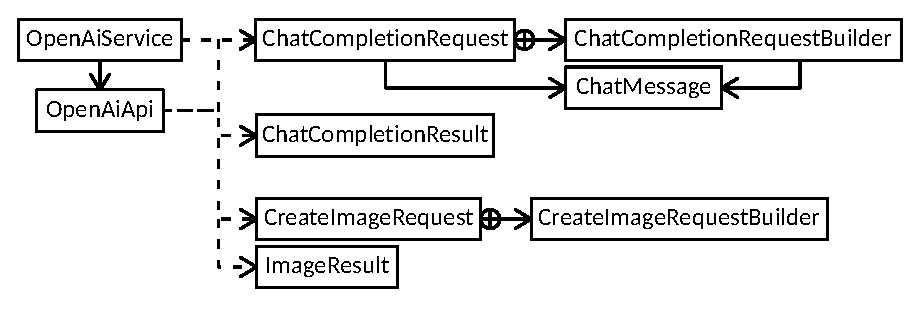
\includegraphics{chapter/chapter_3/mechanisms/openai-endpoint-mech.eps}
    \caption{Endpunkte der OpenAI Schnittstelle.}
    \label{sec3:model:subsubsec:genai-integration:fig:openai-endpoint-comps}
\end{figure}

\cref{sec3:model:subsubsec:genai-integration:fig:openai-endpoint-comps} zeigt ein partielles Klassendiagramm, welches die an der Erstellung von Anfragen an die Endpunkte der Schnittstelle beteiligten Komponenten zeigt.
Die Komponenten \textit{OpenAiService} und \textit{OpenAiApi} bieten Zugriff auf die Funktionalitäten der Schnittstelle und behandeln zudem die Konfiguration der Schnittstelle.
Weitere Komponenten sind \textit{ChatCompletionRequest} und \textit{CreateImageRequest}, die jeweils als Objekt eine Anfrage an einen Endpunkt darstellen.
Die Anfragen müssen dann noch über die Komponente \textit{OpenAiService} an die Schnittstelle gesendet werden.
Analog zu den Anfragen sind die Komponenten \textit{ChatCompletionResult} und \textit{ImageResult} Container, die die Ergebnisse der Anfragen an die jeweiligen Endpunkte speichern.
Folglich bestehen diese Komponenten wiederum aus kleinen weiteren Komponenten, die die jeweiligen Informationen speichern.
Die Komponenten \textit{ChatCompletionRequestBuilder} und \textit{CreateImageRequestBuilder} sind jeweils die Komponenten, die die Parameter der Anfrage spezifizieren.
Inbesondere ist in Bezug auf die Anfragen zur Generierung von Text die Komponente \textit{ChatMessage} von Bedeutung.
Während bei normalen Anfragen, wie z.B. der Anfrage zur Generierung von Bildern nur einfache Texteingaben benötigt werden, wird bei der Anfrage von Text eine Reihe an Textnachrichten (\textit{ChatMessage}) benötigt, die einen Dialog zwischen mehreren Parteien darstellen.
Eine Textnachricht erwartet als Eingabe eine Rolle im Dialog, sowie den Inhalt dieser Partei im Dialog.

Die genannten Komponenten stellen die Grundlage zum Erstellen einer Anfrage an die Endpunkte der Schnittstelle von OpenAI dar.
Im Folgenden ist es nun von Interesse herauszufinden, welche Informationen für das Erstellen einer effektiven und sinnvollen Anfrage an einen Endpunkt der Schnittstelle notwendig sind, und welche Komponenten am Erzeugen dieser Informationen beteiligt sind.
Speziell für die Textgenerierung bestehen die Informationen für den Dialog, der durch eine Reihe an Textnachrichten \textit{ChatMessage} dargestellt wird, zumeist aus Instruktionen (siehe z.B. \cref{sec3:model:subsubsec:explainability-through-genai}), sowie den in Textformat transformierten Informationen aus einem Graph Code (siehe \cref{sec3:model:subsubsec:gc-transformation}).

Der Prozess der Verarbeitung der Informationen eines Graph Codes wird, wie bereits durch das Sequenzdiagramm für den Anwendungsfall \hyperref[sec3:model:uc-1.3]{UC-1.3} dargestellt, von einem Benutzer durch die Auswahl eines Graph Codes initiiert.
Schlussendlich wird dann der Komponente \textit{ExplanationPanel} ein Graph Code übergeben, welche diesen Graph Code dann an die spezifischen Komponenten \textit{ImagePanel} und \textit{TextPanel} der Erklärungstypen \textit{Image} oder \textit{Text} delegiert.
Die Verarbeitung der Informationen erfolgt dann gesondert und abhängig vom Erklärungstyp durch die Komponenten \textit{TextPanel} oder \textit{ImagePanel} in der Methode \textit{setUpPrompt}.
Ein Beispiel für die Zusammenstellung der durch die Transformation generierten Informationen in der Methode \textit{setUpPrompt} kann in folgendem Beispiel eingesehen werden:

\begin{tcolorbox}[enhanced, colback=white,segmentation style={solid}, breakable]
  \textbf{System}: \enquote{You are an assistant, who is able to generate cohesive textual explanations based on a collection of words.}
  \tcbline
  \textbf{Assistant}: \enquote{The collection of words represents a dictionary. The dictionary contains so-called feature vocabulary terms. Some of the dictionary terms are connected through a relationship. These relationships will be noted as $<i_{t}> - <i_{t_{1}},...,i_{t_{n}}>$ or $<i_{t}> k <i_{t_{1}},...,i_{t_{n}}>$, where $i_{t}$ denotes the index of a feature vocabulary term. Additionally $-$ represents an undefined relationship, while $k$ represents a specific relationship.}.
  \tcbline
  \textbf{User}: \enquote{The collections of words is as follows: <\textit{Liste der Merkmale aus dem Wörterbuch eines Graph Codes}>. The relationships are as follows: <\textit{Generierte Formate der Beziehungen durch einen Graph Code}>. Generate a coherent textual explanation containing the terms of the dictionary. An example for such an explanation could be: <\textit{Beispiel zur Verdeutlichung...}>.}.
  \tcbline
  \textbf{Assistant}: \enquote{Based on the dictionary, here is a cohesive textual explanation containing the terms of the dictionary:}.
\end{tcolorbox}

Die Verarbeitung der durch die Transformation generierten Informationen und in einer Prompt zusammengetragenen Informationen wird im Folgenden durch einen allgemeinen \cref{sec3:model:subsubsec:genai-integration:alg:text-end} beschrieben, der die Sequenz der notwendigen Schritte und Aktionen hervorhebt, um eine Anfrage an den Endpunkt Text (\textit{ChatCompletionRequest}) zur Generierung von Text zu erstellen.

% <Pseudoalgorithmus>
\begin{algorithm}[htb]
\caption{Anfrage an den Endpunkt Text (\textit{ChatCompletionRequest}).}
\label{sec3:model:subsubsec:genai-integration:alg:text-end}
\begin{algorithmic}[1]
\Procedure{createRequest}{}
  \State Service initialisieren... (\textit{OpenAiService})
  \State Anfrage initialisieren... (\textit{ChatCompletionRequest})
  \State Anfrage anpassen, Parameter setzen... (\textit{ChatCompletionRequestBuilder})
  \State Anfrage an Schnittstelle senden (\textit{OpenAiService})
  \State Ergebnis erhalten und entsprechend verwerten (\textit{ChatCompletionResult}, \textit{TextPanel})
\EndProcedure
\end{algorithmic}
\end{algorithm}


Bezüglich der Erstellung einer Anfrage an den Endpunkt Bild (\textit{ImageRequest}) zum Generieren eines Bildes besteht allerdings das Problem der Tokenbegrenzung von Dall-E 2.
Im Folgenden wird ein Konzept entwickelt, um diesem Problem zu begegnen.
Dieses Konzept sieht das In-Reihe-Schalten der Endpunkte vor.
Genauer wird zuerst eine Anfrage an den Endpunkt Text zum Generieren von Text erstellt und gesendet, um darauffolgend mit dem daraus resultierenden Ergebnis die Eingabe für eine Anfrage an den Endpunkt Bild zu speisen.
Dies ist möglich, da die Anfrage an den Endpunkt Text spezifisch dazu parametrisiert werden kann, dass das Ergebnis dieser Anfrage nur eine maximale Länge an Zeichen umfassen darf/soll.
Des Weiteren können die Instruktionen der Prompt zur Generierung von Text so angepasst werden, dass dem System generativer KI vermittelt wird, dass das erzeugte Ergebnis dieser Anfrage wiederum als Eingabe für ein Bilderzeugungsprogramm verwendet werden soll (siehe \cref{sec3:model:subsubsec:explainability-through-genai}, \enquote{Create a visual explanation / description.}).
Das Erzeugen einer Anfrage an den Endpunkt Bild verhält sich analog zum Endpunkt Text.

% Beschreibung der Erweiterung...

% Hier wäre es dann vermutlich noch sinnvoll auf die Zusammenstellung der in \cref{sec3:model:subsubsec:gc-transformation} generierten Informationen zu sprechen... Dies würde dann in erster Linie ein Pseudoalgorithmus für die Erstellung einer Anfrage an den Endpunkt Text (ChatCompletionRequest) sein... Gesondert wird dann noch darüber gesprochen, wie das Problem mit der Tokenbegrenzung für den Endpunkt Bild (ImageRequest) gehandhabt werden kann -> Erst Textanfrage mit spezifischen Anfrageparametern (geringe Tokenzahl der Antwort...), dann Bildanfrage (also in Reihe geschalten) (hierfür dann eventuell eine Erweiterung des Pseudoalgorithmus oder nur eine detaillierte Beschreibung des Ablaufs) -> nur eine detaillierte Beschreibung

% Zusammenstellung der generierten Informationen aus der Transformation ansprechen...
% Dies wird in erster Linie ein Pseudoalg für die Erstellung einer Anfrage an den Endpunkt Text sein (ChatCompletionRequest)
% Gesondert sollte dann darüber gesprochen werden, wie das Problem mit der Tokenbegrenzung für den Endpunkt Bild gehandhabt werden kann...
% In Reihe schalten (Text, dann Bild) mit einer spezifischen Textanfrage und passenden Anfrageparametern (geringe Tokenanzahl)
% Nur Beschreibung des Vorgehens für eine Bildanfrage (also Erweiterung nur textuell beschreiben, kein eigener Pseudoalg).

Mit diesen neuen Informationen kann eine Erweiterung bzw. Ergänzung des Sequenzdiagramms für den Anwendungsfall \hyperref[sec3:model:uc-1.3]{UC-1.3} vorgenommen werden.
\cref{sec3:model:par:seq-use-cases:fig:seq-diag-uc-1.3-exp} zeigt die Erweiterung des Sequenzdiagramms um die neuen Abläufe der Verarbeitung von Graph Codes in den Komponenten \textit{ImagePanel} und \textit{TextPanel}.

\begin{figure}[htb]
    \centering
    \resizebox{\textwidth}{!}{
        \begin{tikzpicture}
            \begin{umlseqdiag}
                
                \umlmlobject[x=0, fill=white]{gcs}{\shortstack[c]{Graph Code \\ SelectionListener}}
                \umlmlobject[x=4, fill=white]{ep}{\shortstack[c]{Explanation \\ Panel}}
                \umlmlobject[x=8, fill=white]{imgp}{\shortstack[c]{ImagePanel}}
                \umlmlobject[x=11, fill=white]{txtp}{\shortstack[c]{TextPanel}}

                % Calls
                \begin{umlcall}[padding=0,dt=6,op={Setze Graph Code}]{gcs}{ep}
                    \begin{umlcall}[op={Setze Graph Code}]{ep}{imgp}
                        \begin{umlcallself}[op={\shortstack[c]{Verarbeite\\GraphCode}}]{imgp}
                        \end{umlcallself}
                    \end{umlcall}
                    \begin{umlcall}[dt=4,op={Setze Graph Code}]{ep}{txtp}
                        \begin{umlcallself}[op={\shortstack[c]{Verarbeite\\GraphCode}}]{txtp}
                        \end{umlcallself}
                    \end{umlcall}
                \end{umlcall}
            \end{umlseqdiag}
        \end{tikzpicture}
    }
    \caption{Erweiterung zum Sequenzdiagramm für den Anwendungsfall \hyperref[sec3:model:uc-1.3]{UC-1.3}.}
    \label{sec3:model:par:seq-use-cases:fig:seq-diag-uc-1.3-exp}
\end{figure}

Weitere Parameter zum Anpassen einer Anfrage an einen Endpunkt der Schnittstelle können durch die Benutzerschnittstellen, dargestellt in \cref{sec3:model:par:wireframe:fig:stage-2+3}, generiert werden.
Genauer würden die Spezifikationen der Anfragen an die Endpunkte der Schnittstelle durch die gewählten Einstellungen im Rahmen des Anwendungsfall \hyperref[sec3:model:uc-1.7]{UC-1.7} in den erweiterten Optionen (siehe \cref{sec3:model:par:wireframe:fig:stage-2+3} \circitem{9}) zustande kommen.

Anhand dieser Informationen kann nun auch ein Mechanismus für den Anwendungsfall \hyperref[sec3:model:uc-1.8]{UC-1.8} erstellt werden (siehe \cref{sec3:model:par:mechanism-use-cases:fig:mech-uc-1.8}).
Der Anwendungsfall \hyperref[sec3:model:uc-1.8]{UC-1.8} \enquote{Erklärung generieren} beginnt durch das Klicken des Knopfes \enquote{Generate ...}.
Im weiteren Verlauf erzeugt das System dann die notwendigen Komponenten für eine Anfrage an einen Endpunkt der Schnittstelle.
Diese Objekte werden dann durch durch die in den erweiterten Optionen gewählten Einstellungen parametrisiert und die Anfrage finalisiert.
Schlussendlich übergibt das System die Anfrage an die Komponente \textit{OpenAiService}, welche die Anfrage dann an die Schnittstelle sendet und auf diese Weise eine Erklärung generieren lässt.
Es ist wichtig anzumerken, dass diese Beschreibung für das Generieren von Erklärungen sehr generisch ist und für beide Erklärungstypen gilt.

\begin{figure}[htb]
    \centering
    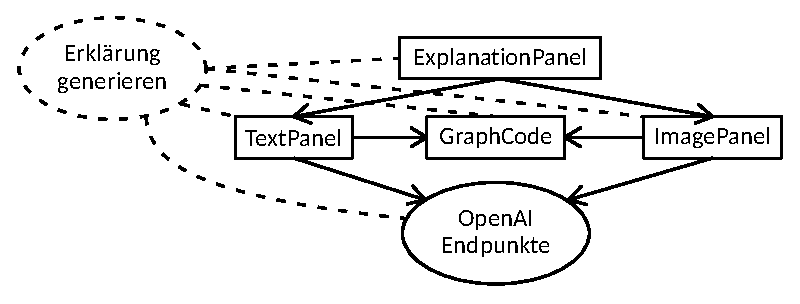
\includegraphics{chapter/chapter_3/mechanisms/mechanism-uc-1.8.eps}
    \caption{Mechanismus für den Anwendungsfall \hyperref[sec3:model:uc-1.8]{UC-1.8}.}
    \label{sec3:model:par:mechanism-use-cases:fig:mech-uc-1.8}
\end{figure}

\begin{figure}[htb]
    \centering
    \resizebox{\textwidth}{!}{
        \begin{tikzpicture}
            \begin{umlseqdiag}
                % Actors
                \umlactor[fill=white, scale=0.7]{Benutzer}

                % Objects
                \umlobject[x=0, fill=white]{Benutzer}
                \umlmlobject[x=3.3, fill=white]{tip}{\shortstack[c]{(Text/Image)Panel}}
                \umlmlobject[x=7, fill=white]{rq}{(...)Request}
                \umlmlobject[x=10, fill=white]{bld}{\shortstack[c]{(...)Request\\Builder}}
                \umlmlobject[x=13, fill=white]{oas}{OpenAiService}


                % Calls
                \begin{umlcall}[padding=0,dt=7,op={\shortstack[c]{Erklärung \\ generieren}}]{Benutzer}{tip}
                    \begin{umlcall}[padding=2.5,op={Erzeuge Anfrage},return={Anfrage}]{tip}{rq}
                    \end{umlcall}
                    \begin{umlcall}[padding=2.5,dt=4,op={Parameter der Anfrage anpassen}, return={Modifizierte Anfrage}]{tip}{bld}
                    \end{umlcall}
                    \begin{umlcall}[padding=2.5,dt=4,op={Anfrage an Endpunkt senden}, return={Ergebnis in Form von (Text/Bild)}]{tip}{oas}
                    \end{umlcall}
                    \begin{umlcallself}[dt=4,op={\shortstack[c]{Ergebnis\\verarbeiten\\/ anzeigen}}]{tip}
                    \end{umlcallself}
                \end{umlcall}
            \end{umlseqdiag}
        \end{tikzpicture}
    }
    \caption{UML-Sequenzdiagramm für den Anwendungsfall \hyperref[sec3:model:uc-1.8]{UC-1.8}.}
    \label{sec3:model:par:seq-use-cases:fig:seq-diag-uc-1.8}
\end{figure}


\cref{sec3:model:par:seq-use-cases:fig:seq-diag-uc-1.8} zeigt ein Sequenzdiagramm für den Anwendungsfall \hyperref[sec3:model:uc-1.8]{UC-1.8}.
Es zeigt, wie der Benutzer die Aktion \enquote{Erklärung generieren} durch einen Klick auf den Knopf \enquote{Generate ...} initiiert.
Die Abbildung stellt dabei eine generische Darstellung eines Ablaufs zum Generieren einer Erklärung dar und gilt für beide Komponenten \textit{ImagePanel} und \textit{TextPanel}.
Im weiteren Verlauf wird dann die notwendigen Komponenten, die für eine Anfrage benötigt werden, erzeugt und anhand von Benutzereingaben parametrisiert bzw. deren Parameter modifiziert.
Hierzu gehören im Übrigen auch die Eingabeaufforderungen / Prompt, die die bereits verarbeiteten Informationen aus einem Graph Code enthalten.
Diese angepasste Anfrage kann dann über den Endpunkt an die Schnittstelle gesendet werden.
Nach Fertigstellung der Verarbeitung seitens des Systems generativer KI, wird über die Schnittstelle ein Ergebnis, abhängig vom Erklärungstyp, zurückgeliefert.
Dieses Ergebnis kann dann schlussendlich von der Komponente \textit{ImagePanel} oder \textit{TextPanel} weiterverarbeitet oder angezeigt werden.

\FloatBarrier

\subsubsection{Diskussion}
\label{sec3:model:subsubsec:fz2:discussion}
In diesem Abschnitt wurden die offenen Herausforderungen \hyperref[sec2:sota:oi:2.1]{\textbf{OH 2.1}} und \hyperref[sec2:sota:oi:2.2]{\textbf{OH 2.2}} adressiert.
In \cref{sec3:model:subsubsec:gc-transformation} wurde die offene Herausforderung \hyperref[sec2:sota:oi:2.1]{\textbf{OH 2.1}} behandelt und Konzepte zur Transformation von Graph Codes vorgestellt, mit welchen Graph Codes in eine geeignete Form zur Eingabe in Systeme generativer KI transformiert werden sollen.
In Abschnitt \cref{sec3:model:subsubsec:genai-integration} wurde die offene Herausforderung \hyperref[sec2:sota:oi:2.2]{\textbf{OH 2.2}} behandelt und Konzepte zur Integration von Systemen generativer KI vorgestellt.

\clearpage

\subsection{Zusammenfassung}
\label{sec3:model:subsec:summary}
In diesem Kapitel wurde die Modellierung behandelt und es wurden in \cref{sec3:model:subsec:fz-explainability} Konzepte für die Erklärbarkeit von MMIR mittels generativer KI, sowie in \cref{sec3:model:subsec:fz-integration} Konzepte für die Integration von generativer KI in das GMAF entwickelt.
In \cref{sec3:model:subsubsec:summary-findings} werden die in diesem Kapitel gewonnen Erkentnisse zusammengefasst, in \cref{sec3:model:subsubsec:futher-approach} wird das weitere Vorgehen festgehalten und schlussendlich in \cref{sec3:model:subsec:summary:table:summary} eine Übersicht des aktuellen Arbeitstands in einer Tabelle dargestellt.

\subsubsection{Gewonnene Erkenntnisse}
\label{sec3:model:subsubsec:summary-findings}
In diesem Abschnitt werden die Erkenntnisse aus den Forschungszielen \enquote{FZ 1.2/TB Erklärbarkeit von MMIR mittels generativer KI} und \enquote{FZ 2.2/TB Integration generativer KI in das GMAF} zusammengefasst.

Im ersten Forschungsziel wurde angesprochen, wie Erklärbarkeit durch generative KI erreicht werden kann.
Darüber hinaus wurden in Bezug auf das GMAF eine Reihe an benutzerorientierten Anwendungsfällen identifiziert und textuell beschrieben.
Anhand dieser Anwendungsfälle wurden schrittweise Benutzerschnittstellen mit geeigneten Interaktionsmöglichkeiten konzipiert.
Des Weiteren wurden mit Hilfe von Mechanismen, die an Anwendungsfällen beteiligten Komponenten identifiziert, anhand derer wiederum Sequenz- bzw. Interaktionsdiagramme und Pseudoalgorithmen erstellt werden konnten.

Im zweiten Forschungsziel wurde die Transformation der in Graph Codes gespeicherten, sowie der mit Graph Codes assoziierten Informationen behandelt und es wurden Konzepte zur Überführung dieser Informationen in eine geeignete Form, den Prompts, in Systeme generativer KI entwickelt.
Zusätzlich wurde die Einbindung der Systeme generativer KI in das GMAF behandelt und Konzepte zur Integration dieser in das GMAF entwickelt.

Die in den \cref{sec3:model:subsec:fz-explainability,sec3:model:subsec:fz-integration} gewonnenen Erkenntnisse münden in folgendem Klassendiagramm (siehe \cref{sec3:model:subsec:summary:fig:class-diagram}), in welchem die identifizierten und für die Modellierung wichtigen Klassen, sowie die Beziehungen in denen sie zueinander stehen übersichtlich dargestellt werden.

\begin{figure}[htb]
  \centering
  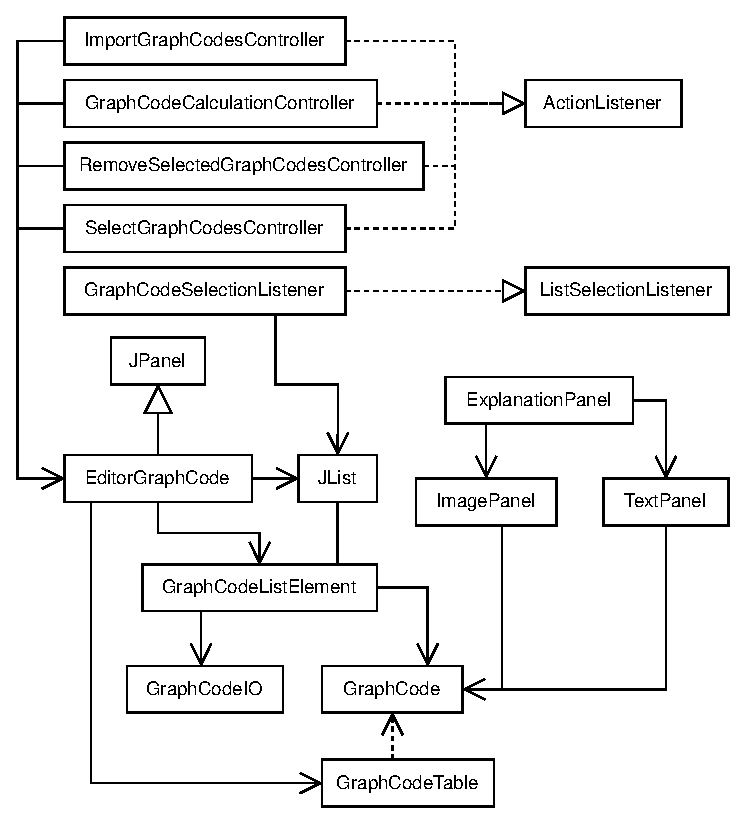
\includegraphics[width=0.8\textwidth]{chapter/chapter_3/class.eps}
  \caption{Klassendiagramm.}
  \label{sec3:model:subsec:summary:fig:class-diagram}
\end{figure}

\FloatBarrier

\subsubsection{Weiteres Vorgehen}
\label{sec3:model:subsubsec:futher-approach}
Im folgenden Kapitel werden die in diesem Kapitel entwickelten Konzepte im Rahmen einer Implementierung durch ihre entsprechenden Forschungsziele untersucht.
Genauer werden in \cref{sec4:impl} in FZ 1.3/I Benutzerschnittstellen und Funktionen implementiert und in FZ 2.3/I die Integration der Systeme generativer KI, sowie die Überführung der Informationen von und um Graph Codes zur Generierung von Erklärungen umgesetzt.

Die nachfolgende Tabelle stellt eine Erweiterung der \cref{sec2:sota:subsec:summary:table:summary} dar und gibt eine Übersicht über den aktuellen Arbeitsstand nach Abschluss dieses Kapitels.

\begingroup
\def\arraystretch{1.1}%
\begin{xltabular}{\linewidth}{
            @{}
            >{
                \hsize=0.2\linewidth
                \raggedright\arraybackslash
            }X
            >{
                \hsize=0.6\linewidth
                \raggedright\arraybackslash
            }X
            >{
                \hsize=0.2\linewidth
            }X
            @{}
        }

        % First Header

        \caption{Tabelle zur Übersicht des aktuellen Arbeitstands.}
        \label{sec3:model:subsec:summary:table:summary}
        \\

        \toprule
        \multicolumn{3}{
            >{
                    \hsize=\linewidth\centering\arraybackslash
            }X
        }
        {
            \textbf{Forschungsziele}
        } \\ \midrule
        \textbf{FZ / OH} &  \textbf{Beschreibung} & \textbf{Referenz} \\ \midrule

        \endfirsthead

        \toprule
        \multicolumn{3}{
            >{
                    \hsize=\linewidth\centering\arraybackslash
            }X
        }
        {
            \textbf{Forschungsziele}
        } \\ \midrule
        \textbf{FZ / OH} & \textbf{Beschreibung} & \textbf{Referenz} \\ \midrule

        \endhead

        % Lower Rows

        \multicolumn{3}{
            >{
                    \hsize=\linewidth\centering\arraybackslash
            }X
        }
        {
            \textbf{Erklärbarkeit von MMIR mittels generativer KI}
        }
        \\
        \midrule

        FZ 1.1/O
        &
        Recherche zur Erklärbarkeit von MMIR mittels generativer KI
        \\

        &
        Grundlegende Technologien:
        &

        \\

        &
        \tabitem GMAF
        &
        \cref{sec2:sota:subsubsec:gmaf}
        \\

        &
        \tabitem MMFG
        &
        \cref{sec2:sota:subsubsec:mmfg}
        \\

        &
        \tabitem Graph Code
        &
        \cref{sec2:sota:subsubsec:graph-codes}
        \\

        % Offene Herausforderungen aus FZ1/O

        OH 1.1
        &
        Erste offene Herausforderung
        &
        \hyperref[sec2:sota:oi:1.1]{\textbf{OH 1.1}}
        \\


        &
        Systeme generativer KI und ein Überlick über aktuelle Systeme
        &
        \cref{sec2:sota:subsubsec:genai}
        \\

        &
        Diskussion und Auswahl von Systemen
        &
        \cref{sec2:sota:subsubsec:fz1:discussion}
        \\

        OH 1.2
        &
        Zweite offene Herausforderung
        &
        \hyperref[sec2:sota:oi:2.1]{\textbf{OH 2.1}}
        \\

        \midrule

        FZ 1.2/TB
        &
        Modellierung der Erklärbarkeit von MMIR mittels generativer KI
        &

        \\

        &
        Erklärbarkeit durch generative KI
        &
        \cref{sec3:model:subsubsec:explainability-through-genai}
        \\

        &
        $\rightarrow$ Behandlung der ersten offenen Herausforderung \hyperref[sec2:sota:oi:1.1]{\textbf{OH 1.1}}
        &
        \\

        &
        Anwendungsfälle:
        &
        \cref{sec3:model:subsubsec:use-cases}
        \\

        &
        \tabitem Textuelle Beschreibungen
        &
        %\cref{sec3:model:par:textual-desc-use-cases}
        \\

        &
        \tabitem Wireframes
        &
        %\cref{sec3:model:par:wireframe}
        \\

        &
        \tabitem Mechanismen
        &
        %\cref{sec3:model:par:mechanism-use-cases}
        \\

        &
        \tabitem Sequenzdiagramme
        &
        %\cref{sec3:model:par:seq-use-cases}
        \\

        &
        $\rightarrow$ Behandlung der zweiten offenen Herausforderung \hyperref[sec2:sota:oi:1.2]{\textbf{OH 1.2}}
        &
        \\

        \midrule

        FZ 1.3/I
        &
        Implementierung der Erklärbarkeit von MMIR mittels generativer KI
        &

        \\

        \midrule

        FZ 1.4/E
        &
        Evaluierung der Erklärbarkeit von MMIR mittels generativer KI
        &

        \\

        \midrule

        \multicolumn{3}{
            >{
                    \hsize=\linewidth\centering\arraybackslash
            }X
        }
        {
            \textbf{Integration generativer KI in das GMAF}
        }
        \\
        \midrule

        FZ 2.1/O
        &
        Recherche zur Integration generativer KI in das GMAF
        &

        \\


        &
        Aufzeigen der Integrationsmöglichkeiten von:
        &

        \\

        &
        \tabitem Graph Codes
        &
        \cref{sec2:sota:subsubsec:gc-capabilities-integration}
        \\

        &
        Erste offene Herausforderung
        &
        \hyperref[sec2:sota:oi:2.1]{\textbf{OH 2.1}}
        \\

        &
        \tabitem Systemen generativer KI
        &
        \cref{sec2:sota:subsubsec:genai-capabilities-integration}
        \\

        &
        Zweite offene Herausforderung
        &
        \hyperref[sec2:sota:oi:2.2]{\textbf{OH 2.2}}
        \\

        \midrule

        FZ 2.2/TB
        &
        Modellierung der Integration generativer KI in das GMAF
        &

        \\

        &
        Transformation von Graph Codes
        &
        \cref{sec3:model:subsubsec:gc-transformation}
        \\

        &
        \tabitem Transformation des Vokabulars
        &
        \\

        &
        \tabitem Transformation der Matrix
        &
        \\

        &
        \tabitem Anwendung von Graph Code Metriken
        &
        \\

        &
        $\rightarrow$ Behandlung der ersten offenen Herausforderung \hyperref[sec2:sota:oi:2.1]{\textbf{OH 2.1}}
        &
        \\

        &
        Einbindung generativer KI in das GMAF
        &
        \cref{sec3:model:subsubsec:genai-integration}
        \\

        &
        $\rightarrow$ Behandlung der zweiten offenen Herausforderung \hyperref[sec2:sota:oi:2.2]{\textbf{OH 2.2}}
        &
        \\

        \midrule

        FZ 2.3/I
        &
        Implementierung der Integration generativer KI in das GMAF
        &

        \\

        \midrule

        FZ 2.4/E
        &
        Evaluierung der Integration generativer KI in das GMAF
        &

        \\

        \bottomrule
\end{xltabular}
\endgroup

